\documentclass[a4paper,11pt]{book}
% Layout
% Gráficos e layout

\ifx\pdfmatch\undefined
\else
    \usepackage[T1]{fontenc}
    \usepackage[utf8]{inputenc}
\fi

% xetex:
\ifx\XeTeXinterchartoks\undefined
\else
    \usepackage{fontspec}
    \defaultfontfeatures{Ligatures=TeX}
\fi

% luatex:
\ifx\directlua\undefined
\else
    \usepackage{fontspec}
\fi

% End engine-specific settings

% Fonte
%\usepackage{lmodern}
\usepackage{times}

% Pacotes adicionados
\usepackage{ae}
% Língua e hifenização
\usepackage[portuguese]{babel}
\usepackage{hyphenat}
\usepackage{hyperref} % Permite Links personalizados
\usepackage{fancyhdr}
\usepackage{sectsty}
\usepackage{float}   % Gerencia melhor o posicionamento das figuras e tabelas
%\usepackage{graphicx}
\usepackage[pdftex]{color,graphicx}
\usepackage{hyperref}
\usepackage{enumerate} % Permite alterar Layout do enumerate
\usepackage{enumitem}  % Permite opções de {itemize}
%\usepackage{pdflscape}  % Permite alterar a orientação da pagina para Paisagem
%\usepackage{ifthen}  % Permite usar condicionais ifelse
\usepackage{xcolor} %cores
\usepackage{amsmath,amssymb} % Ambiente para uso de elementos matemáticos
\usepackage{caption}
\usepackage{subcaption} % permite o uso de multiplas figuras com legenda (ambiente subfigure)
\usepackage{minted} % Ambiente para blocos de código
\usepackage{natbib} % Para referencia bibliográfica
\usepackage{url}    % Referência de links na internet
%\usepackage{listings} % pacote para apresentar código de programação
\usepackage{indentfirst}  % Para indentar o primeiro parágrafo de cada seção
\usepackage{titling}  % Permite Montar uma página de titulo própria
\usepackage{tcolorbox} % Caixas Coloridas com Bordas =D
\usepackage{multicol} % Permite colocar textos e imagens lado a lado

% Layout do documento

% Bordas e tamanho da página
\usepackage{geometry} 
 \geometry{ % Padrõa ABNT para relatórios
 a4paper,
 left=30mm,
 right=20mm,
 top=30mm,
 bottom=20mm
 }

% Cabeçalho e Rodapé
\pagestyle{fancy} % https://www.sharelatex.com/learn/Headers_and_footers
  \lhead{}
  \chead{}
  \rhead{Projeto Edubot} % cabeçalho margem direita
  \lfoot{}
  \cfoot{}
  \rfoot{\thepage} % rodapé margem direita

% Numeração
  \pagenumbering{arabic}

% Retas do cabeçalho e rodapé
  \renewcommand{\headrulewidth}{0.5pt}
  \renewcommand{\footrulewidth}{0.5pt}

% Tamanho da letra
    \chapterfont{\huge}
    \sectionfont{\Large}
    \subsectionfont{\large}

% Hiperlinks
\hypersetup{
    colorlinks,
    citecolor=black,
    filecolor=black,
    linkcolor=black,
    urlcolor=black
}

% Definições do pdf
\hypersetup{
    unicode=false,          % non-Latin characters in Acrobat’s bookmarks
    pdftoolbar=true,        % show Acrobat’s toolbar?
    pdfmenubar=true,        % show Acrobat’s menu?
    pdffitwindow=false,     % window fit to page when opened
    pdfstartview={FitH},    % fits the width of the page to the window    
    pdfauthor={Projeto Edubot - UnB},     % author
    pdfnewwindow=true      % links in new window
}

% Outros
%\renewcommand{\thesection}{(\alph{section})} % muda o estilo de númeração das sections
% alterando a formatação dos numeradores de lista de itens
\renewcommand\theenumi{\arabic{enumi}}
\renewcommand\labelenumi{\textbf{\alph{enumi})}}
\renewcommand\theenumii{\arabic{enumii}}
\renewcommand\labelenumii{(\textit{\theenumi.\theenumii})}

% Blocos de questões
%   referência:
%   https://tex.stackexchange.com/questions/66154/how-to-construct-a-coloured-box-with-rounded-corners#66156
% Contador para enumerar as questões
\newcounter{question}[subsection]
% Define caixas para formatação
\newtcolorbox{questionbox}[1]{
    colback=blue!5!white, 
    colframe=blue!75!black,
    fonttitle=\bfseries,
    title=#1
}
\newtcolorbox{chalengebox}[1]{
    colback=red!5!white,
    colframe=red!75!black,
    fonttitle=\bfseries,
    title=#1
}
% Formatar questões
\newcommand{\question}[1]{\stepcounter{question}\noindent
\begin{questionbox}{Exercício \thesection.\thequestion\hspace{0.2cm}}
#1
\end{questionbox}}
% Formatar questões de desafio mantendo a numeração
\newcommand{\challenge}[1]{\stepcounter{question}\noindent
\begin{chalengebox}{\thesection.\thequestion\hspace{0.2cm} Desafio}
#1
\end{chalengebox}}
\newcommand{\FNada}[1]{#1}

\def\BibTeX{{\rm B\kern-.05em{\sc i\kern-.025em b}\kern-.08em
    T\kern-.1667em\lower.7ex\hbox{E}\kern-.125emX}}
% permite que o comando \underline{\hspace{.1in}} escreva um underline

\usepackage[document]{ragged2e}


\title{Apostila didática}
\author{Projeto Edubot}

% Documento
\begin{document}
% Capa da apostila
\begin{figure}[h!]
    \centering
    
\includegraphics[scale=0.9]{Figuras/simb_unb.png}
    \label{fig:unb}
    \caption*{Universidade de Brasília}
\end{figure}

\begin{center}
    Departamento de Engenharia Elétrica
    
    Capitulo Estudantil IEEE de Robótica e Automação (IEEE - RAS UnB)
    
    Projeto Edubot
    
    \vfill
    
    \Huge \bf \thetitle
    
    \vfill
    
    \large % fonte
    
    Brasília \\
    \the\year % Coloca o Ano atual
    
    \thispagestyle{empty} % Retira o cabeçalho e o rodapé da página
\end{center}

% Cabeçalho
\newpage
Incluir aqui um cabeçalho para o aluno preencher seu nome, sua escola e alguns dados pessoais.
\tableofcontents
\newpage


\chapter*{Como usar esta apostila?}
   Explicar o objetivo da apostila para qualquer pessoa que pegar ela para ler. Além disso, explicar aos alunos como devem utilizá-la ao longo de seus estudos.

\chapter{Afinal, o que é um robô?}
\section*{Introdução}
\paragraph{}
O desejo de solucionar problemas do dia-a-dia de maneira mais eficiente e simples, foi - e ainda é - um dos maiores promotores para o desenvolvimento tecnológico das mais diversas sociedades. De acordo com a necessidade de cada período, cientistas (engenheiros, matemáticos, físicos, etc) de diferentes povos propunham maquinários e ferramentas que pudessem operar em conjunto com outros seres vivos para \textbf{modificar} a forma de trabalho, melhorando a qualidade de vida dos trabalhadores e das suas famílias. Com isso, impulsionou-se a busca por maiores níveis de \textbf{automação}, consequentemente levando às tentativas de aplicar esse conceito no cotidiano, sendo esse o patamar que alcançamos e presenciamos nos dias atuais.\\

É nesse contexto que a ideia da utilização de robôs para a realização de diversas tarefas acabou se popularizando, colocar uma máquina para completar uma tarefa muito trabalhosa ou difícil e assim poupar trabalho humano é um dos focos da robótica. O robozinho utilizado como material de estudo no nosso curso é o \textit{Sparki}, ele é uma dessas máquinas que tem como objetivo facilitar a nossa vida, nesse caso o ensino de programação, mas o que difere ele e outros robôs de um ar condicionado ou um projetor? \par

\section{Para que estudar a definição de robô?}

\paragraph{}
Como descrito na introdução desse capítulo, a robótica está presente em diversos aspectos do nosso cotidiano. Dentre as mais diversas aplicações existentes, podemos listar algumas:

\begin{itemize}
\item Culinária, robôs que auxiliam na preparação de pratos e na entrega dos mesmos em restaurantes (segue-linha);

\item Robôs industriais, como carregados (segue-linha), robôs montadores de peças em indústrias;

\item Robôs cirúrgicos, como o Star (tecidos moles mais delicados), o PRECEYES (áreas delicadas, como os olhos), CorPath (operações cirúrgicas a distância através do Wifi), The Monarch Platform (broncoscopia, i.e. intervenção cirúrgica nos brônquios), Mako Rio (auxiliar em implante em joelhos e costela), Versius (cirurgias não invasivas);

\item Robôs para comunicação com crianças;

\item Robôs de exploração espacial, como o Hover em Marte;

\item Robô para inspecionar de tubulações;

\item Robô para serviços de casa (seja de superfícies aquáticas, ou terrestres). Exemplos: Row-bot, Ro-Boat, Roomba.
\end{itemize}

    \begin{figure}[h]
    \caption{Exemplo de um robô, o Roomba}
     
    \centering 
    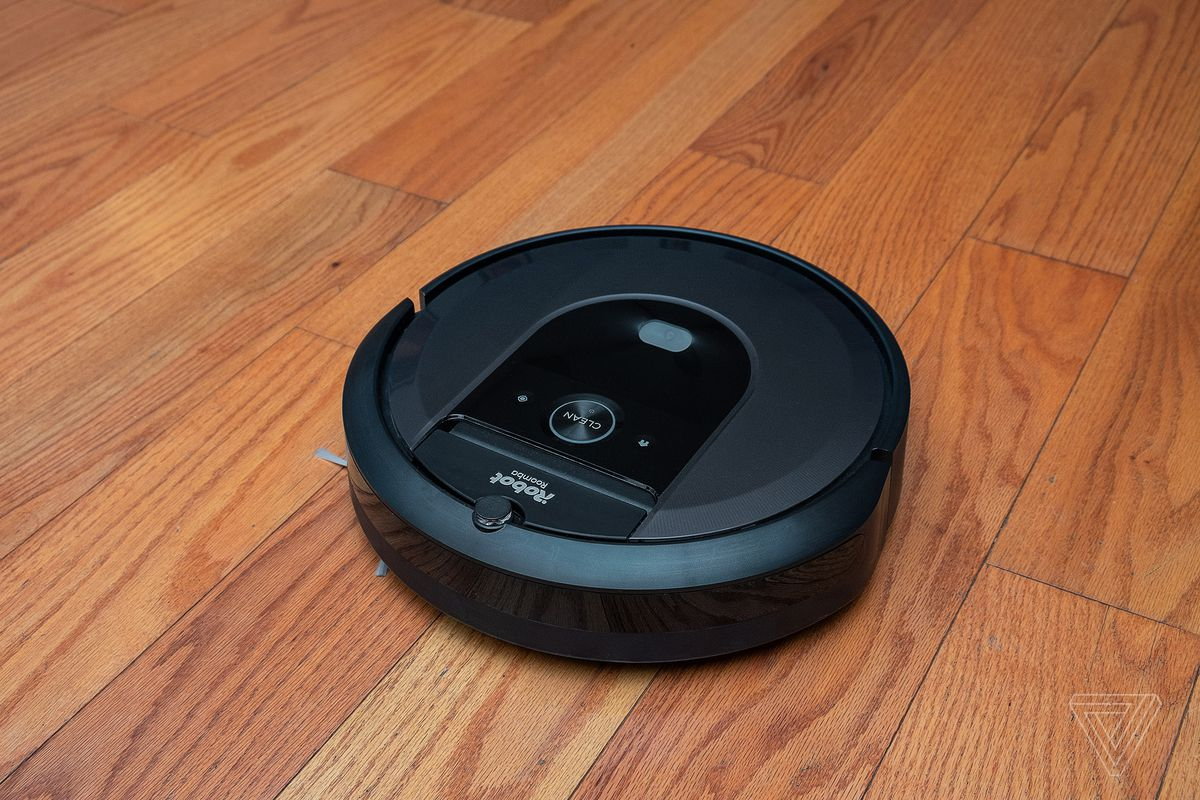
\includegraphics[width=8cm]{Figuras/roomba.jpg}
    \label{figura:roomba.jpeg}
    \end{figure}
 

\section{Definindo um robô}
\paragraph{}
Para uma máquina ser considerada um robô, a primeira coisa que ela deve ser capaz de fazer é raciocinar de alguma maneira.\\

\textit{Como assim, um robô tem que ser capaz de pensar assim como nós (pessoas)?} \par
Não necessariamente, algo assim é muito complexo e difícil de acontecer... Quando dizemos que um robô deve raciocinar, queremos dizer que ele deve ter a capacidade de analisar o mundo ao seu redor e tomar decisões a partir do que ele analisou, ele precisa agir em função do seu ambiente. Um robô segue linhas por exemplo, necessita de algum sensor que permita a ele encontrar a localização da linha e a partir dai decidir como irá se movimentar sobre ela e o que fazer caso perca a linha de vista. De maneira geral, a ação realizada pelos robôs normalmente é algum tipo de movimento, alguma atividade mecânica como andar ou mover algo, um semáforo que acende a luz vermelha para os carros para possibilitar a passagem de pedestres após ter seu botão apertado não é considerado um robô, uma porta automática de um shopping se aproximaria mais do que é um robô.\\

\textit{Qual a relevância deste assunto no mundo? Afinal, para que mesmo eu estou lendo esta apostila? Eu sei que eu vou ganhar um diploma do curso, mas... E aí? O que mais que isso aqui pode me acrescentar?}\par
Nosso curso busca ajudar os alunos a entender de forma simples como que um robô, um computador ou outros equipamentos raciocinam, como que nós pessoas somos capazes de criar linhas de pensamento para coisas não pensantes. Nós mostraremos que a programação não é um bicho de sete cabeças e forneceremos a base necessária para que vocês cheguem mais preparados e entusiasmados em algum curso superior, técnico ou trabalho que aborde programação.

\begin{center}

    \textbf{Definição}
    
    \justify
    Um robô é uma máquina \textbf{autônoma}, que existe no \textbf{mundo físico}, possui \textbf{sensores} para perceber o ambiente e consegue \textbf{agir} sobre o meio para alcançar um ou mais objetivos definidos.
\end{center}

\paragraph{}
Nós já falamos sobre os sensores e conseguir agir sobre o meio, mas e os outros requisitos?
Existir no mundo físico nada mais é do que algo que somos capazes de tocar e manipular, uma bola de futebol por exemplo existe no mundo físico, os sonhos que temos ao dormir não existem no mundo físico, pois não somos capazes de tocá-lo.
Uma máquina autônoma ou automática, é uma máquina que após ligada ela funciona sozinha sem a constante necessidade de interferência externa, ela ainda pode aceitar o aperto de botões ou o recebimento de outros tipos de comandos, mas a ideia é que ela seja capaz de realizar tarefas sozinha quando for necessário.

\section*{Para saber mais}

\begin{enumerate}
    \item Mais informações sobre o sistema robótico PRECEYES estão disponíveis em:

    \url{https://www.brabantbrandbox.com/life-sciences/preceyes/}. Acesso em 13 de Agosto de 2019.
    
    \item Quer saber um pouco mais sobre os procedimentos cardíacos auxiliados pelo CorPath? Acesse: https://www.corindus.com/
    \item Mais informações sobre The Monarc Plataform em:


    https://www.aurishealth.com/monarch-platform.
    \item Mais informações sobre o Mako Rio em: \\
    \url{https://www.stryker.com/us/en/portfolios/orthopaedics/joint-replacement/mako}
    \url{-robotic-arm-assisted-surgery.html}.
    \item Assista o próprio Jonathan Rossiter falando sobre o Rowbot em:
    
    \url{https://www.youtube.com/watch?v=KCL8NjN7FMQ}.
    
    \item Mais informações sobre o Ro-boat em:
    http://roboat.org/.
    \item Introdução à robótica - Maja Mataric. \\
    \url{https://web.icmc.usp.br/SCATUSU/Boletim_aquisicao/Boletim_novembro_2016/Capas_novembro_2016/Mataric_Introducao0001.pdf}
\end{enumerate}

\section{Exercícios}

\question{Além das aplicações citadas nesse capítulo, pesquise mais 3 áreas em que a robótica está presente.}

\begin{center}
    \line(1,0){450}
    \vspace{0.2cm}   
    \line(1,0){450}
    \vspace{0.2cm}   
    \line(1,0){450}
    \vspace{0.2cm}   
    \line(1,0){450}
    \vspace{0.2cm}   
\end{center}

\question{Um termômetro pode ser considerado um robô dentro da definição vista neste capítulo? Justifique.}

\begin{center}
    \line(1,0){450}
    \vspace{0.2cm}   
    \line(1,0){450}
    \vspace{0.2cm}   
    \line(1,0){450}
    \vspace{0.2cm}   
\end{center}

\question{Cite 3 exemplos de robôs dentro da cultura popular (filmes, séries, \textit{animes} etc.) que são erroneamente considerados robôs.}

\begin{center}
    \line(1,0){450}
    \vspace{0.2cm}   
    \line(1,0){450}
    \vspace{0.2cm}
\end{center}

\question{Dentre os aparelhos eletrônicos presentes em sua casa, quais deles mais se assemelha às características que definem um robô?}

\begin{center}
    \line(1,0){450}
    \vspace{0.2cm}   
    \line(1,0){450}
    \vspace{0.2cm} 
\end{center}

\challenge{
    {\large{Desafio:}} Escolha algum dos exemplos de robôs apresentados ou algum outro do seu interesse e procure entender a lógica de seu funcionamento (quais os seus sensores, qual a lógica por trás de suas ações).
}

\begin{center}
    \line(1,0){450}
    \vspace{0.2cm}   
    \line(1,0){450}
    \vspace{0.2cm}   
    \line(1,0){450}
    \vspace{0.2cm}   
    \line(1,0){450}
    \vspace{0.2cm}   
\end{center}
\chapter{Algoritmos e tela LCD}
\section*{Introdução}
    Neste capítulo veremos o que significa algoritmo, o que é uma tela LCD e para que ela serve. Além disso, vamos abordar o conceito de linguagem de programação e saber, afinal, como nos comunicar com o \textit{Sparki}. E aí, vamos nessa?
\section{Algoritmo}
    Diariamente utilizamos algoritmos sem mesmo perceber. Quando cozinhamos um macarrão, assamos um bolo, montamos um móvel, um brinquedo ou mesmo quando escovamos os dentes estamos utilizando este conceito para completar essas tarefas. \par
    Isto porque tomamos essas decisões nos baseando em instruções claras para chegar a um objetivo. Então, se estamos preparando um bolo, não podemos simplesmente colocar os ingredientes no forno sem antes misturá-los conforme a receita. Não teríamos um bolo, mas um Frankestein! Da mesma forma, não poderíamos esperar que ele fique pronto se ligarmos o forno, mas não colocássemos a massa do bolo nele. \par
    \begin{center}
    \textbf{Definição} \\
    Algoritmo é um conjunto finito de instruções sequenciais lógicas, bem definidas, não ambíguas que levam à solução de um problema.
    \end{center}
    \textit{Mas afinal o que esse bando de palavras complicadas querem dizer ? Eu não entendi foi nada.}
    
    O que elas querem dizer é, em outras palavras, que um algoritmo indica um conjunto de instruções para realizar uma tarefa qualquer, como por exemplo, fazer pipoca. Seguimos uma receita que nos diz bem direitinho o que fazer para atingir o objetivo desejado, que no caso é aquela pipoca bem quentinha e crocante no final das contas! Assim ficou mais fácil de entender, né? \par
    Como já vimos, robôs não raciocinam como nós, seres humanos. Então precisamos deixar bem claro o que esperamos de cada um deles quando estamos nos comunicamos com eles para que o objetivo final seja cumprido. 
    
    \textit{Ué, mas isto parece exatamente com algo que você já disse.}  
    
    Exatamente! Escrevemos algoritmos para fazer a programação de robôs! \par 
    Até agora vimos que algoritmos são extremamente importantes e é essencial que o seu conceito seja entendido. Mas você sabia que não precisamos de um computador para programar?
\subsection{Torre de copos}
    Desafio torre de copos.


\section{Linguagem de programação}
    Se fosse dado o comando abaixo para o \textit{Sparki} você acha que ele entenderia? \par
    \begin{center}
    \textit{Sparki vai para frente! Sparki vai para trás!}\ \par
    \end{center} \par
    Quem pensou que ele não entenderia acertou, o \textit{Sparki} não iria entender nada do que foi dito. \par
    \textit{Então como ele entende os comandos que pedimos para ele fazer?}\par
    Para nos comunicarmos com o \textit{Sparki}, é preciso passar os comandos para o computador através de uma linguagem de programação, que irá converter o que escrevemos para zeros e uns e depois enviará para \textit{Sparki}, e assim ele será capaz de entender e executar o comando.
    
    \begin{center}
    \textbf{Definição} \\
    Uma linguagem de programação é um método padronizado para comunicar instruções para um computador.
    \end{center} \par
    
 
\subsection{Funções importantes: \textit{void setup(), void loop()}}
    
    A biblioteca  \textit{sparki.h} e as funções \textit{void setup e void loop} são as funções mais importantes na hora de começar a programar o \textit{Sparki}, pois entender o que elas significam e como funcionam é essencial para saber onde escrever determinada parte do código em relação ao tipo de aplicação.
    
    \begin{minted}{cpp}
    #include <Sparki.h>
    void setup()
    {
    }
    void loop()
    {
    }
    \end{minted}

    \begin{itemize}
        \item Biblioteca \textit{sparki.h}: Esta biblioteca guarda todas as funções relacionadas ao \textit{Sparki}, e é necessário inserir ela na primeira linha de código, para que estas funções sejam habilitadas para a comunicação entre o computador e o robô funcionar.
        \item \textit{Void Setup()}: Esta função é a primeira a rodar no código, e tudo que está dentro de suas chaves é executado apenas uma vez. A função é bastante útil para inserir configurações iniciais, como por exemplo limpar a tela LCD, ou fazer algum movimento inicial que não irá se repetir no resto do programa.
        \item \textit{Void Loop}: Esta função é usada para colocar códigos que irão ficar se repetindo no programa, ou seja, sempre ficará rodando até que seja carregado algum outro programa no \textit{Sparki}. Um exemplo para esta função é deixar o \textit{Sparki} sempre com o LED de uma cor ligado, ou sempre se movimentando em uma determinada direção.
        \end{itemize}
    
  %  Escrever código de como mostrar algo na tela do Sparki

\section{Tela de LCD (\textit{Liquid Crystal Display})}
O \textit{Sparki} possui uma tela LCD onde é possível desenhar, escrever e visualizar dados de sensores em funcionamento. A tela é formada por \textit{pixels}, que são pequenos pontos de luz que podem estar ligados ou desligados para formar uma imagem. No caso do \textit{Sparki}, ele possui 128 \textit{pixels} na horizontal e 64 \textit{pixels} na vertical, e para identificar cada pixel deve ser fornecido a coordenada horizontal, vertical, e se ele deverá ficar aceso ou apagado. \par
\textit{Então toda vez que eu for escrever algo no LCD preciso fazer a coordenada de cada pixel?}
Não, porque alguém já disse ao computador como ligar e desligar pixels para formar os caracteres, ou seja, se você quer escrever uma letra 'A' por exemplo, já está armazenado quais pixels devem acender e apagar para que a tela mostre exatamente a letra 'A'.

\section{Exercícios}
\question{Em suas palavras, defina o que é uma linguagem de programação.}
    Deixar espaço de linhas.
    \vspace{4cm}        % Espaçamento vertical
    
\question{O objetivo de uma linguagem de programação é:}
    \begin{enumerate}
        \item Fornecer um conjunto de regras bem definidas que permita escrever programas de computador de forma mais amigável evitando ambiguidades.
        \item Dar a liberdade para cada programador escrever programas de computador a partir do seu próprio conjunto de regras, facilitando o processo de programação.
        \item Estabelecer regras para comunicação entre seres humanos.
        \item Definir um padrão para programadores utilizarem os comandos binários intrínsecos a cada arquitetura de processador.
    \end{enumerate}

\subsection{}

\subsection{}

\subsection{}

\subsection{\large{Desafio:}}
% Capítulo Movimentação =========================================
\chapter{Tela de LCD (\textit{Liquid Crystal Display})}

    \begin{figure}[h]
    \caption{Tela LCD}
     
    \centering 
    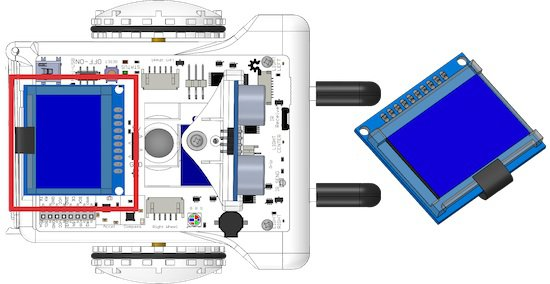
\includegraphics[width=9cm]{Figuras/Top_LCD1.jpeg}
    \label{figura:Top_LCD1.jpeg}
    \end{figure}

\section*{Introdução}
\paragraph{}
O \textit{Sparki} possui uma tela LCD onde é possível desenhar, escrever e visualizar dados de sensores em funcionamento. Ao olhar bem de perto, pode-se perceber que a tela é formada por pequenos pontos que podem ser programados para estarem em um de dois estados, ligado ou desligado. Nós chamamos esses pontos de \textit{pixels}. Eles também estão presentes em TVs, monitores de computador, celulares e eles são ligados ou desligados em uma disposição na qual seja possível formar uma imagem na tela. No caso do \textit{Sparki}, ele possui 128 \textit{pixels} na horizontal e 64 \textit{pixels} na vertical, e para identificar cada pixel deve ser fornecido a coordenada horizontal, vertical, e se ele deverá ficar aceso ou apagado. 

    \begin{figure}[h]
    \caption{Pixels}
     
    \centering 
    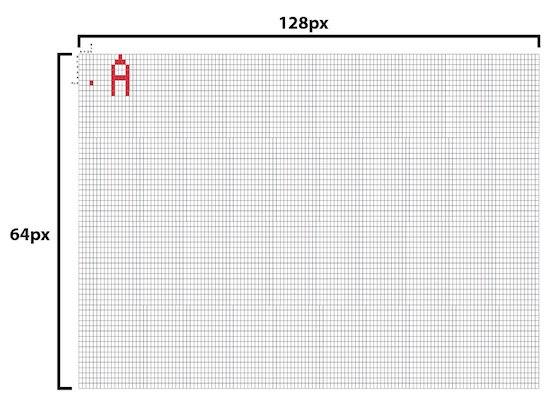
\includegraphics[width=9cm]{Figuras/LCD_Diagram1.jpg}
    \label{figura:LCD_Diagram1.jpg}
    \end{figure}
    
\section{Funções}

Para imprimir algo na tela LCD, você deve seguir 4 passos importantíssimos:
\begin{description}
\item[1.] Limpar o LCD --> \lstinline[columns=fixed]{sparki.clearLCD()}
\item[2.] Informar o que você quer que apareça no LCD -->
%não consegui arrumar a identação do código aqui. Talvez essa função não funcione bem dentro de tópicos.
\begin{lstlisting}[language=C]
sparki.drawLine(x,y,127,63);
sparki.drawRect(5,5, 30,10); 
sparki.drawRectFilled(15,17,30,10); 
sparki.drawCircle(20,45,12); 
sparki.drawCircleFilled(90,40,20); 
sparki.print("nao pula linha"); 
sparki.println("pula linha depois");
\end{lstlisting}

\item[3.] Atualizar a tela --> \lstinline[columns=fixed]{sparki.updateLCD()}
\item[4.] Criar um intervalo de tempo --> \lstinline[columns=fixed]{delay()}
\end{description}

\subsection{Passo 1: Limpar o LCD}

\paragraph{}
O primeiro passo para mostrar algo no LCD é limpar todas as informações que estão no armazenadas no \textit{Sparki} e, para isso, utilizamos a função \lstinline[columns=fixed]{sparki.clearLCD()}. Esta função não precisa de parâmetros, então não precisamos escrever nada dentro dos parênteses.

\begin{center}
    \textcolor{mydarkblue}{\textbf{Para não esquecer!}} 
    \\ ``Clear'' traduzido para o português significa ``limpar''.
\end{center}

\subsection{Passo 2: Informar ao LCD}

\paragraph{sparki.drawLine(xi, yi, xf, yf):} 
Esta função cria uma linha de acordo com o ponto de início e do fim do traço. Então \lstinline[columns=fixed]{xi} e \lstinline[columns=fixed]{yi} são as coordenadas do ponto de início do traço e \lstinline[columns=fixed]{xf} e \lstinline[columns=fixed]{yf} são as coordenadas do fim do traço.

\paragraph{sparki.drawRect(xi, yi, xf, yf):}
Esta função desenha um retângulo, sendo \lstinline[columns=fixed]{xi} e \lstinline[columns=fixed]{yi} coordenadas do canto superior esquerdo do retângulo e \lstinline[columns=fixed]{xf} e \lstinline[columns=fixed]{yf} coordenadas do canto inferior direito do retângulo.

\paragraph{sparki.drawRectFilled(xi, yi, xf, yf):}
Esta função é semelhante à \lstinline[columns=fixed]{sparki.drawRect(xi, yi, xf, yf)}, a única diferença é que ele desenha um retângulo preenchido.
 
\paragraph{sparki.drawCircle(xc, yc, raio):}
Esta função desenha um círculo de acordo com as coordenadas do centro e o raio. As coordenadas \lstinline[columns=fixed]{xc} e \lstinline[columns=fixed]{yc} indicam onde deve ficar o centro do círculo e o parâmetro \lstinline[columns=fixed]{raio} indica o tamanho do raio.
 
\paragraph{sparki.drawCircleFilled(xc, yc, raio):}
Esta função é semelhante à \lstinline[columns=fixed]{sparki.drawCircle(xc, yc, raio)}, a única diferença é que ele desenha um círculo preenchido.

\begin{center}
    \textcolor{mydarkblue}{\textbf{Para não esquecer!}} 
    \\ ``Draw'' traduzido para o português significa ``desenhar''.
    \\ ``Line'' traduzido para o português significa ``linha''.
    \\ ``Rect'' é uma abreviação de ``rectangle'', que traduzido para o português significa ``retângulo''.
    \\ ``Circle'' traduzido para o português significa ``círculo''.
    \\ ``Filled'' significa ``preenchido''.
\end{center}

\paragraph{sparki.print:} 
Com esta função, é possível imprimir caracteres e números na tela, basta escrever a mensagem a ser impressa dentro dos parênteses e das aspas. Essa função também é bastante utilizada para imprimir os valores recebidos dos sensores, mas, para essa utilidade, o parâmetro deverá ser uma variável* e o nome dela não será escrita entre aspas.
\par* No capítulo 5 iremos aprender mais sobre variáveis e seus usos, por isso, não vamos nos ater muito à funcionalidade do sparki.print(variavel), ok?
  
\paragraph{sparki.println:}
Assim como a função anterior, ela imprime uma mensagem na tela. A diferença é que essa função gera uma quebra de linha ao fim dessa mensagem.

\begin{center}
    \textcolor{mydarkblue}{\textbf{Para não esquecer!}} 
    \\ ``Print'' traduzido para o português significa ``imprimir''.
\end{center}

\subsection{Passo 3: Atualizar a tela do LCD}

\paragraph{}
A função \lstinline[columns=fixed]{sparki.updateLCD()} é importante para atualizar a tela, informando ao \textit{Sparki} que ele já pode mostrar no LCD as informações que foram passadas.

\begin{center}
    \textcolor{mydarkblue}{\textbf{Para não esquecer!}} 
    \\ ``Update'' traduzido para o português significa ``atualizar''.
\end{center}

\subsection{Passo 4: Criar um intervalo de tempo}
\paragraph{}
Para criar um intervalo de tempo, devemos utilizar a função \lstinline[columns=fixed]{delay()}. Ela não precisa de parâmetros.\\

\textit{Não entendi o porquê de precisarmos criar um intervalo de tempo. Não faz sentido!} \par
O intervalo de tempo é necessário para que a mensagem/imagem permaneça na tela por tempo suficiente para que possamos visualizá-la. Caso criemos um código para o LCD sem incluir esse passo, não conseguiremos visualizar na tela. Ficou confuso? Basta pensar que estamos limpando e atualizando o LCD com novas informações o tempo todo, então, os \textit{pixels} estão sendo ligados e desligados a cada vez que o \lstinline[columns=fixed]{void loop()} é lido. Por isso, queremos que as informações continuem sendo exibidas na tela (\lstinline[columns=fixed]{sparki.updateLCD()}) por mais tempo do que elas permanecem apagadas (\lstinline[columns=fixed]{sparki.clearLCD()}).

\begin{center}
    \textcolor{mydarkblue}{\textbf{Para não esquecer!}} 
    \\ ``Delay'' traduzido para o português significa ``demora'', ``atraso''.
\end{center}

\subsection{Exemplos}
\textsc{Exemplo 1)} Neste exemplo a tela LCD do \textit{Sparki} irá mostrar duas retas, uma partindo do canto superior esquerdo e indo até o canto inferior direito e outra partindo do canto superior direito e indo até o canto inferior esquerdo. E esse desenho será mostrado no LCD por 1 segundo antes do código ser repetido.

\begin{lstlisting}[language=C]
#include <Sparki.h>;

void setup()
{
}

void loop()
{
    sparki.clearLCD();
    sparki.drawLine(0,0,127,63);
    sparki.drawLine(0,63,127,0);        
    sparki.updateLCD();
    delay(1000);  
}
\end{lstlisting}

\textsc{Exemplo 2)} Agora vamos fazer um exemplo com o círculo preenchido. Neste caso, o raio do círculo é 10 e as coordenadas são as seguintes: x = 60, y = 30;

\begin{lstlisting}[language=C]
#include <Sparki.h>;

void setup()
{
}

void loop()
{
  sparki.clearLCD();
  sparki.drawCircleFilled(60,30,10);
  sparki.updateLCD();
  delay(1000);  
}
\end{lstlisting}

\textsc{Exemplo 3)} Neste exemplo, iremos visualizar um código que imprime um retângulo. 


\begin{lstlisting}[language=C]
#include <Sparki.h>;

void setup()
{
}

void loop()
{
  sparki.clearLCD();
  sparki.drawRect(10,15,20,25);
  sparki.updateLCD();
  delay(1000);  
}
\end{lstlisting}

Para começar, vamos analisar os parâmetros da função de desenhar um retângulo. Os dois primeiros parâmetros representam as coordenadas do ponto referente ao canto superior esquerdo, ou seja, xi = 10, yi = 15. Já os dois últimos, eles fazem referência ao ponto do canto inferior direito, ou seja, xf = 20, yf = 25. Note que a ordem dos parâmetros faz muita diferença quando se trata de funções.
\\~\\
\par \textsc{Exemplo 4)} Agora, veremos um exemplo de como imprimir caracteres na tela LCD por meio de aspas.
\begin{lstlisting}[language=C]
#include <Sparki.h>;

void setup()
{
}

void loop()
{
  sparki.clearLCD();
  sparki.println("Oi, eu sou o Sparki");
  sparki.print("Tudo bem");
  sparki.print("?");
  sparki.updateLCD();
  delay(1000);  
}
\end{lstlisting}

Perceba que em um dos comandos de imprimir caracteres tem um "ln", lembra o que isso significa? Isso significa que, após escrever os caracteres que estão entre as aspas, será pulada uma linha. Então ficaria mais ou menos assim:

\begin{table}[h]
 \centering
 {\renewcommand\arraystretch{1.5}
 \caption{Resultado no LCD}
 \begin{tabular}{ l }
  \cline{1-1}  
    \multicolumn{1}{|p{3.333cm}|}{Oi, eu sou o Sparki       Tudo bem?}
  \\  
  \hline
 \end{tabular} }
\end{table}

\section{Exercícios}

\question{Crie um código que desenhe no centro da tela LCD do Sparki um círculo de raio 20 e, no centro dele, um círculo preenchido de raio 10. Dica: lembre-se das proporções dessa tela LCD.}
    \begin{center}
    \line(1,0){450}
    \vspace{0.2cm}   
    \line(1,0){450}
    \vspace{0.2cm}   
    \line(1,0){450}
    \vspace{0.2cm}   
    \line(1,0){450}
    \vspace{0.2cm}   
    \line(1,0){450}
    \vspace{0.2cm}   
    \line(1,0){450}
    \vspace{0.2cm}   
    \line(1,0){450}
    \vspace{0.2cm}   
    \line(1,0){450}
    \vspace{0.2cm}   
    \line(1,0){450}
    \vspace{0.5cm}   
    \end{center}

\question{Marque qual das alternativas é equivalente à mensagem que será exibida na tela do \textit{Sparki} após o seguinte código ser lido:}

\begin{lstlisting}[language=C]
#include <Sparki.h>;

void setup()
{
}

void loop()
{
  sparki.clearLCD();
  sparki.print("Ola ");
  sparki.println("humanos!");
  sparki.print("Eu me");
  sparki.print("chamo ");
  sparki.println("Sparki");
  sparki.updateLCD();
  delay(1000);  
}
\end{lstlisting}

\begin{enumerate}
        \item Ola humanos!Eu me chamo Sparki
        \item Ola \\
        humanos! Eu me chamo \\
        Sparki
        \item Ola humanos! \\
        Eu me chamo Sparki
        \item Ola humanos! \\
        Eu mechamo Sparki
    \end{enumerate}

\question{Responda qual seria a altura e o comprimento do retângulo impresso na tela LCD (em pixels), com base no seguinte código:}

\begin{lstlisting}[language=C]
#include <Sparki.h>;
void setup()
{
}
void loop()
{
  sparki.clearLCD();
  sparki.drawRect(10,15,35,25);
  sparki.updateLCD();
  delay(1000);  
}
\end{lstlisting}

a) Altura do retângulo:
\begin{center}
    \line(1,0){450}
    \vspace{0.3cm}   
\end{center}
b) Comprimento do retângulo:
\begin{center}
    \line(1,0){450}
    \vspace{0.5cm}   
\end{center}

\challenge{Crie um código que imprima um rosto na tela LCD do Sparki, de forma que os olhos sejam círculos preenchidos e a boca seja um retângulo. As proporções ficam a seu critério.}
\begin{center}
    \line(1,0){450}
    \vspace{0.2cm}   
    \line(1,0){450}
    \vspace{0.2cm}   
    \line(1,0){450}
    \vspace{0.2cm}   
    \line(1,0){450}
    \vspace{0.2cm}   
    \line(1,0){450}
    \vspace{0.2cm}   
    \line(1,0){450}
    \vspace{0.2cm}   
    \line(1,0){450}
    \vspace{0.2cm}   
    \line(1,0){450}
    \vspace{0.2cm}   
    \line(1,0){450}
    \vspace{0.5cm}   
\end{center}

\chapter{Movimentação}
\section*{Introdução}
    \paragraph{}
    Será neste capítulo que iremos aprender a movimentar o \textsl{Sparki}, os comandos para ele ir para frente, rotacionar e realizar todos os percursos que a nossa imaginação puder criar. Para isso, será necessário utilizar as funções a seguir.
    
\section{Funções}
    \paragraph{}
    Todas as funções desse capítulo começam com \lstinline[columns=fixed]{sparki.move}, você consegue pensar em um motivo para a palavra ``move'' estar em destaque?\\
    
    \textit{Move... Mover... Movimentar...} \par
    Exatamente! Movimentação é a resposta, pois ``move'' significa ``se movimentar'' em inglês.

\subsection{sparki.moveForward(int distancia);}
    \paragraph{}
    Essa é a principal função de movimentação, pois é um comando para o robô ``andar'' para frente. Sendo ``distancia'' uma variável que representa quantos centímetros o \textsl{Sparki} deverá se movimentar para frente. Após ter percorrido essa distância, ele passará a executar a próxima linha de comando, ou seja, a próxima ação.\\
    
    \textit{Variável? Mas o que é essa tal de variável?} \par
    Não se preocupe! Teremos um capítulo inteiro apenas para entendê-la, mas, por enquanto, iremos utilizá-la para informar ao \textsl{Sparki} qual a distância em centímetros que queremos que ele percorra, ou os ângulos em graus que queremos que ele rotacione. Simples assim!\\
    
    \textit{E o que significa esse `int' dentro dos parênteses?} \par
    Ele indica que o número que colocaremos dentro dos parênteses tem que ser um número inteiro.
    
    \begin{center}
    \textcolor{mydarkblue!80!black}{\textbf{Lembrando:}} Números inteiros são aqueles que não têm a parte decimal, ou seja, não possuem vírgula. $\mathbb{Z}=\{..., -3, -2, -1, 0, 1, 2, 3, ...\}$.
    \end{center}
    
    \paragraph{}
    Como queremos que o \textsl{Sparki} vá para frente, além de ser um número inteiro, tem que ser positivo também! Ah! Se não tiver escrito nada no espaço entre os parênteses, o \textsl{Sparki} irá para frente indefinidamente, ou seja, até que seja lida a função \lstinline[columns=fixed]{sparki.moveStop()}, ou até que a bateria dele acabe...
    \paragraph{}
    Parece complicado, mas vou dar um exemplo passo a passo para você ver que não é.
    \\~\\
    \textsc{Exemplo 1)} Vamos supor que o seu objetivo é fazer o \textsl{Sparki} andar para frente.
    
    \begin{itemize}
        \item O primeiro passo é identificar a função a ser utilizada para o \textsl{Sparki} andar para frente, neste caso, \lstinline[columns=fixed]{sparki.moveForward(int distancia)};
        \item O segundo passo é decidir o qual vai ser o valor a ser escrito entre os parênteses, ou seja, o parâmetro dessa função. Como não determinamos uma distância, pois queremos que ele ande para frente e não pare, não é necessário escrever um número, basta deixar em branco. O valor default é 1, logo, escrever \lstinline[columns=fixed]{sparki.moveForward()} é o mesmo que escrever \lstinline[columns=fixed]{sparki.moveForward(1)};
        \item Agora que sabemos a função e o seu parâmetro, podemos aplicar no código. Ficaria assim:
    \end{itemize}
    
    \begin{lstlisting}[language=C]
#include <Sparki.h>;

void setup()
{
}

void loop()
{
    sparki.moveForward();
}
\end{lstlisting}
    
    \paragraph{}
    Quando queremos passar uma informação para outra pessoa, podemos falar de diversas formas, seja de um jeito mais devagar ou até muito rápido, bem formal ou com várias gírias. Então, pode-se dizer que, independente do modo com que falamos, a pessoa irá entender a informação, mas, dependendo da pessoa com quem falamos, devemos escolher o modo mais conveniente. Por exemplo, não podemos falar da mesma forma com os nossos amigos e com o/a diretor/a do colégio, para este último devemos tentar utilizar uma linguagem mais formal. Na programação isso também acontece, existem vários códigos diferentes que fazem basicamente a mesma coisa, mas sempre devemos escolher o mais eficiente ou conveniente para cada caso.
    \\~\\
    \textsc{Exemplo 2)} Vamos aproveitar para ver um código que faz o mesmo que o do \textsc{Exemplo 1}. Outra forma de fazer o robô andar para frente sem parar seria escrevendo um número qualquer como parâmetro \lstinline[columns=fixed]{sparki.moveForward(int distancia)}.
    
    \begin{lstlisting}[language=C]
#include <Sparki.h>;

void setup()
{
}

void loop()
{
    sparki.moveForward(100);
}
\end{lstlisting}
    
    \textit{Como assim?? Você disse que o número que vinha dentro dos parênteses determinava a distância. Então, se eu colocar um número qualquer, o \textsl{Sparki} vai parar depois de andar a distância escrita, não?} \\
    Sim, o número dentro dos parênteses indica sim a distância a ser percorrida, mas há algo que você pode estar se esquecendo. Tente se lembrar da definição de \lstinline[columns=fixed]{void loop()}. Ela falava que tudo o que estiver escrito dentro das chaves do \lstinline[columns=fixed]{void loop()} seria repetido várias e várias vezes, até que a bateria do robô acabe. Como só existe uma função dentro do loop, essa vai se repetir para sempre, é como se o \textsl{Sparki} estivesse andando 100 centímetros para frente e, depois que terminasse, mais 100 centímetros para frente e depois mais 100 centímetros para frente... Essa sequência ficaria se repetindo, sem parar.
    
    \paragraph{}
    Bom, chegamos a conclusão de que o \textsc{Exemplo 1} e o \textsc{Exemplo 2} são códigos que geram a mesma ação, agora devemos pensar em qual seria mais eficiente ou conveniente na hora de escrever. Geralmente, optamos pelo código mais simples, sem elementos desnecessários, para que quem estiver lendo possa compreender melhor o nosso código. Logo, o \textsc{Exemplo 1} seria a melhor escolha.
    
    \begin{center}
    \textcolor{mydarkblue}{\textbf{Para não esquecer!}} \\``Forward'' traduzido para o português significa ``para frente''. 
    \end{center}

\subsection{sparki.moveBackward(int distancia);}
    \paragraph{}
    Parecida com a anterior, essa função é utilizada para que o \textsl{Sparki} ``ande'' para trás, sem fazer giros. Sendo ``distancia'' uma variável que representa quantos centímetros ele deverá se movimentar para trás. Da mesma forma que o \lstinline[columns=fixed]{sparki.moveForward()}, se não for escrito nada no espaço entre os parênteses, o \textsl{Sparki} irá para trás indefinidamente, ou seja, até que seja lida a função \lstinline[columns=fixed]{sparki.moveStop()}.
    \\~\\
    
    \textsc{Exemplo 1)} Nesse exemplo, veremos um código que faz o \textsl{Sparki} andar 1 metro para frente e 1 metro para trás.
    
    \begin{itemize}
        \item As funções necessárias são: \lstinline[columns=fixed]{sparki.moveForward(int distancia)}, para andar para frente, e \lstinline[columns=fixed]{sparki.moveBackward(int distancia)}, para andar para trás;
        \item A distância é de 1 metro, mas como o valor tem que ser em centímetro, devemos transformar de metro para centímetros. Substituindo os parâmetros, as funções ficariam assim: \lstinline[columns=fixed]{sparki.moveForward(100)}, \lstinline[columns=fixed]{sparki.moveBackward(100)}.
        \item Agora é só escrever em forma de código!
    \end{itemize}
    
    \begin{lstlisting}[language=C]
#include <Sparki.h>;

void setup()
{
}

void loop()
{
    sparki.moveForward(100);
    sparki.moveBackward(100);
}
\end{lstlisting}
    
    \paragraph{}
    Também poderíamos inserir a função \lstinline[columns=fixed]{delay(int tempo)} entre as funções de movimentação para que o \textsl{Sparki} realize melhor esses movimentos.\\
    
    \textit{O que essa função \lstinline[columns=fixed]{delay(int tempo)} faz mesmo?} \par
    Ela estabelece um tempo de intervalo entre as ações, simplificando, o \textsl{Sparki} espera um tempo determinado pela variável ``tempo'' antes de executar a próxima ação, com isso, podemos acompanhar melhor a execução dos movimentos que escrevemos no nosso código.\\
    
    \textsc{Exemplo 2)} Agora, iremos reescrever o código anterior utilizando a função \lstinline[columns=fixed]{delay(int tempo)} para que, antes do \textsl{Sparki} mudar o sentido do seu movimento, ele dê uma pausa de 3 segundos.
    
    \begin{lstlisting}[language=C]
#include <Sparki.h>;

void setup()
{
}

void loop()
{
    sparki.moveForward(100);
    delay(3000);
    sparki.moveBackward(100);
    delay(3000);
}
\end{lstlisting}
    
    \textit{Por que existem dois \lstinline[columns=fixed]{delay(3000)} no código?}
    
    O primeiro é necessário para estabelecer um intervalo entre andar para frente e andar para trás. O segundo serve para estabelecer um intervalo entre andar para trás e andar para frente, porque, como as funções estão dentro do \lstinline[columns=fixed]{void loop}, depois de \lstinline[columns=fixed]{sparki.moveBackward(100)} o próximo movimento seria \lstinline[columns=fixed]{sparki.moveForward(100)}, então, devemos colocar uma pausa ali também.  
    
    \begin{center}
        \textcolor{mydarkblue!80!black}{\textbf{Lembrando:}} No exemplo anterior nós utilizamos a palavra ``sentido'' no enunciado. Mas você se lembra o que realmente significa esse conceito? E qual a diferença entre ``sentido'' e ``direção''? Vou dar um exemplo para você não errar mais na hora de diferenciar os dois.
    \end{center}
    
    \paragraph{}
    Vamos supor que você saiu de casa e ficou perdido no meio da cidade apenas com a sua pulseira da sorte e uma bússola para te auxiliar a voltar para casa. Essa bússola vai indicar a direção sul, norte, leste, oeste e as várias direções de acordo com os 360 graus dela. Você tem o conhecimento de que a sua casa fica para o sul, por isso, começa a andar nessa direção, saindo da cidade e indo para sua casa. Alguns minutos depois você chega ao seu destino, mas percebe que a sua pulseira caiu no meio do caminho. Então você decide ir de novo para a cidade, pela mesma direção que você veio na volta, mas no sentido contrário ao que você utilizou para voltar para casa, ou seja, saindo da sua casa e indo para a cidade. 
    \paragraph{}
    Contada a história, vamos refletir. A direção pode ser simplificada como uma reta que liga a cidade à sua casa e esta reta possui dois sentidos, o de ida e o de volta. Então, quando estamos falando de uma direção, para facilitar, imagine uma linha tracejada entre o local inicial e o seu ponto de destino. Quando estamos falando de sentidos, pense nessa linha como uma seta (casa -> cidade) para a ida e (cidade -> casa) para a volta.

    \begin{center}
    \textcolor{mydarkblue}{\textbf{Para não esquecer!}} \\ ``Backward'' traduzido para o português significa "para trás".
    \end{center}
    
    \begin{figure}[h]
    \caption{Movimentação Básica}
     
    \centering 
    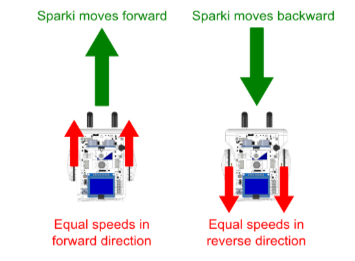
\includegraphics[width=9cm]{Figuras/movimentation_for_back.png}
    \label{figura:movimentation_for_back.png}
    \end{figure}
    
\subsection{sparki.moveStop();}
    \paragraph{}
    Esse é um comando para o \textsl{Sparki} parar de se movimentar, independente do que ele estiver fazendo. Observe que não é necessário escrever nada dentro dos parênteses, o robô irá parar de realizar a ação que ele estiver fazendo no momento em que esse comando for lido.
    
    \begin{center}
        \textcolor{mydarkblue!80!black}{\textbf{Lembrando:}} O tempo a ser escrito como parâmetro, dentro dos parênteses, deve estar em milissegundos.
    \end{center}
    
    \textsc{Exemplo 1)} Neste próximo exemplo, faremos o \textsl{Sparki} andar para frente por 2 segundos e parar, repetidamente.
    
    \begin{itemize}
        \item Primeiro vamos identificar as funções a serem utilizadas para o \textsl{Sparki} andar para frente, esperar 2 segundos e parar. Como vimos no exemplo anterior, a função \\ \lstinline[columns=fixed]{sparki.moveForward(int distancia)} será responsável por andar para frente. Para esperar 2 segundos, devemos utilizar a função \lstinline[columns=fixed]{delay(int tempo)}. Por último, utilizaremos a função \lstinline[columns=fixed]{sparki.moveStop()}, com o objetivo de fazer o \textsl{Sparki} parar.
        \item Agora, vamos decidir os parâmetros dessas 3 funções. Como queremos que o robô ande durante 2 segundos, a função \lstinline[columns=fixed]{sparki.moveForward(int distancia)} será escrita antes da \lstinline[columns=fixed]{sparki.moveStop()}. O \textsl{Sparki} deverá andar por 2 segundos, logo, essa função deverá ser escrita entre as duas anteriores.
        \item Aplicando em código temos:
    \end{itemize}
    
    \begin{lstlisting}[language=C]
#include <Sparki.h>;

void setup()
{
}

void loop()
{
    sparki.moveForward();
    delay(2000);
    sparki.moveStop();
}
\end{lstlisting}
    
    O uso da função \lstinline[columns=fixed]{delay(int tempo)} é de suma importância para o movimento funcionar, sem ela, as funções de andar para frente e parar entrarão em conflito.
    
    \begin{center}
    \textcolor{mydarkblue}{\textbf{Para não esquecer!}}
    \\``Stop'' traduzido para o português significa ``Parar''.
    \end{center}
    
\subsection{sparki.moveRight(int graus);}

    \paragraph{}
    Um pouco diferente dos anteriores, esse é um comando de girar para a direita. Sendo ``graus'' uma variável que representa a variação em graus do giro. Se este campo ficar em branco, o \textsl{Sparki} executará um giro de 90° para a direita.
    \\~\\
    
    \begin{figure}[h]
    \caption{Rotação do Sparki}
     
    \centering 
    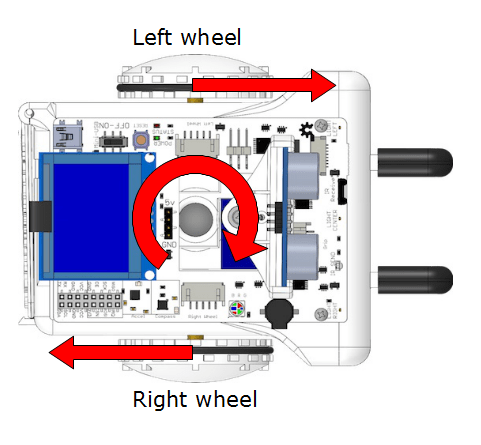
\includegraphics[width=7cm]{Figuras/rotation.png}
    \label{figura:rotation.png}
    \end{figure}
    
    \textsc{Exemplo 1)} Neste código, o \textsl{Sparki} executará um giro à direita de 90° e ficará parado por 1 segundo antes de executar novamente o giro.
    
    \begin{itemize}
        \item As funções necessárias são: \lstinline[columns=fixed]{sparki.moveRight(int graus)} para girar para a direita e \lstinline[columns=fixed]{delay(int tempo)} para gerar uma pausa;
        \item Substituindo os parâmetros, as funções ficariam assim: \lstinline[columns=fixed]{sparki.moveRight()}, pois 90° é o mesmo que deixar em branco, e \lstinline[columns=fixed]{delay(1000)}.
        \item Escrevendo em forma de código:
    \end{itemize}
    
    \begin{lstlisting}[language=C]
#include <Sparki.h>;

void setup()
{
}

void loop()
{
    sparki.moveRight();
    delay(1000);
}
\end{lstlisting}
    
    \begin{center}
    \textcolor{mydarkblue}{\textbf{Para não esquecer!}}
    \\``Right'' traduzido para o português significa ``Direita'', mas lembre-se que não é um deslocamento para direita, e sim um giro.
    \end{center}
    
\subsection{sparki.moveLeft(int graus);}
    \paragraph{}
    Esta função é responsável pelo giro para a esquerda do \textsl{Sparki}. Sendo ``graus'' uma variável que representa a variação em graus do giro. Se este campo ficar em branco, o \textsl{Sparki} executará um giro de 90° para a esquerda.
    \\~\\
    \textsc{Exemplo 1)} Neste exemplo, nós criaremos um código que fará o \textsl{Sparki} realizar um giro completo para a direita, esperar 1 segundo, realizar um giro completo para a esquerda e esperar mais 1 segundo antes que ele repita a sequência.
    
    \begin{itemize}
        \item As funções necessárias são: \lstinline[columns=fixed]{sparki.moveRight(int graus)} para girar para a direita, \lstinline[columns=fixed]{sparki.moveLeft(int tempo)} para girar para a esquerda, além da \lstinline[columns=fixed]{delay(int tempo)} para o intervalo;
        \item Para completar um giro, é necessário realizar os 360 graus, por isso, esse número deve ser escrito dentro dos parênteses das funções de girar. Com o objetivo de fazer uma pausa de 1 segundo, devemos escrever 1000 dentro dos parênteses da função de pausa. Substituindo os parâmetros, as funções ficariam assim: \lstinline[columns=fixed]{sparki.moveRight(360)}, \lstinline[columns=fixed]{sparki.moveLeft(360)}, \lstinline[columns=fixed]{delay(1000)}.
        \item Escrevendo em forma de código:
    \end{itemize}
    
    \begin{lstlisting}[language=C]
#include <Sparki.h>;

void setup()
{
}

void loop()
{
    sparki.moveRight(360);
    delay(1000);
    sparki.moveLeft(360);
    delay(1000)
}
\end{lstlisting}

    \textsc{Exemplo 2)} Que tal juntarmos a função de andar para frente e girar para a esquerda? O código a seguir faz \textsl{Sparki} ir e voltar em uma linha reta. Os movimentos passo a passo são os seguintes: ir para frente por 0,1 metro, esperar 1 segundo parado, girar para a esquerda 180 graus e esperar 1 segundo parado antes de repetir.

\begin{lstlisting}[language=C]
#include <Sparki.h>;

void setup()
{
}

void loop()
{
    sparki.moveForward(10);
    delay(1000);
    sparki.moveLeft(180);
    delay(1000)
}
\end{lstlisting}
    
    \begin{center}
   \textcolor{mydarkblue}{\textbf{Para não esquecer!}}
   \\``Left'' traduzido para o português significa ``Esquerda'', mas lembre-se que não é um deslocamento para esquerda e sim um giro.
    \end{center}
    
    \begin{figure}[h]
    \caption{Sparki fazendo uma curva}
     
    \centering 
    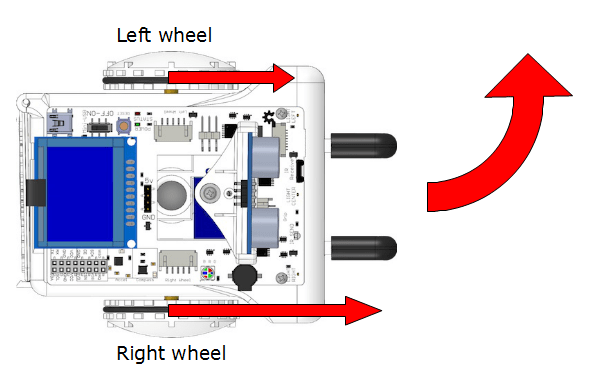
\includegraphics[width=7cm]{Figuras/movingTheRobotmoveLeft.png}
    \label{figura:movingTheRobotmoveLeft.png}
    \end{figure}
    
\subsection{sparki.motorRotate(int motor, int direcao,  int velocidade);}

Quer aprofundar um pouco mais o seu conhecimento sobre movimentação? Então vamos nessa!
\paragraph{}
Sabemos que o \textsl{Sparki} possui duas rodas, mas, para que elas possam rotacionar e fazer o robô se movimentar, tem que existir algo gerando um movimento de rotação. E quem se ocupa dessa tarefa é o motor. Como são duas rodas, existem dois motores, um do lado de cada roda. Para padronizar, iremos chamar o motor do lado direito de ``MOTOR\_RIGHT'' e o motor do lado esquerdo de ``MOTOR\_LEFT''. Agora já sabemos que tem um motor para gerar o movimento, mas, além disso, é necessário decidimos mais duas coisas: qual será a direção para onde ele irá girar e qual será a velocidade dessa rotação. Exitem duas direções de rotação, uma seria o sentido horário e outra o sentido anti-horário, elas serão chamadas respectivamente de: ``DIR\_CW'' e ``DIR\_CCW''.
\paragraph{}
Pronto! Acabamos de aprender os três parâmetros necessários para utilizar a função \lstinline[columns=fixed]{sparki.motorRotate(int motor, int direção, int velocidade)}. No lugar da variável ``motor'' utilizaremos ``MOTOR\_RIGH' se quisermos movimentar o motor e, consequentemente, a roda direita ou ``MOTOR\_LEFT'' se quisermos movimentar a roda esquerda. E no lugar variável ``direcao'' devemos escrever ``DIR\_CW'', sentido do relógio, ou ``DIR\_CCW'', sentido contrário ao do relógio, mas temos que escolher esses dois com cuidado, pois os motores estão virados para fora. Por exemplo, para o motor direito andar para frente, ele utiliza o sentido do relógio, já para o esquerdo, deve-se utilizar o sentido contrário ao do relógio.\\

\textit{Não entendi nada... Se as duas rodas devem andar para frente, por quê um motor utiliza o sentido do relógio e o outro o contrário dele?}\par
Porque o parâmetro ``direcao'' não se refere à direção para onde as rodas estão indo, e sim para que sentido elas estão girando. Tente imaginar o \textsl{Sparki} desmontado, o motor da esquerda estará apontando para a esquerda e o motor da direita estará pontando para a direita, por esse motivo, as direções de rotações serão invertidas. 
\paragraph{}
Faça o teste: vamos supor que os seus dedos são as rodas e as suas mãos os motores. Cruze as mãos e aponte o dedo da mão direita para a direita e o dedo da mão esquerda para a esquerda, olhe no sentido de fora para dentro (ponta da unha -> mão) de cada dedo e gire os dedos no sentido do relógio. Ao fazer o movimento, você perceberá que se o seu dedo que aponta para a direita fosse uma roda, ela estaria andando para frente, mas, se o seu dedo que aponta para a esquerda fosse uma roda, esta estaria andando para trás.
\paragraph{}
Já a terceira variável, ``velocidade'', deve ser substituída por um número entre 0 e 100, sendo 0 a velocidade mínima e 100 a velocidade máxima.
\\~\\
\textsc{Exemplo 1)} Agora um exemplo bem simples para você entender. Utilizaremos a função de rotação do motor para realizar uma ação semelhante à que fizemos no início do capítulo: fazer o \textsl{Sparki} andar para frente por um tempo indeterminado.
        
\begin{itemize}
    \item A função a ser utilizada é \lstinline[columns=fixed]{sparki.motorRotate(int motor, int direcao, int } \\ \lstinline[columns=fixed]{velocidade)}.
    \item Devemos prestar bastante atenção neste momento. Nosso objetivo é fazer o \textsl{Sparki} andar para frente, logo, o motor da direita, ``MOTOR\_RIGHT'', deverá rotacionar no sentido do relógio, ``DIR\_CW'', enquanto o motor da esquerda, ``MOTOR\_LEFT'', deverá rotacionar no sentido contrário ao do relógio, ``DIR\_CCW''. E o parâmetro \lstinline[columns=fixed]{int velocidade} pode ser 75.
    \item Ficará assim:
\end{itemize}
    
    \begin{lstlisting}[language=C]
#include <Sparki.h>;

void setup()
{
}

void loop()
{
    sparki.motorRotate(MOTOR_LEFT, DIR_CCW, 75);
    sparki.motorRotate(MOTOR_RIGHT, DIR_CW, 75);
}
\end{lstlisting}

\begin{center}
    \textcolor{mydarkblue!80!black}{\textbf{Lembrando:}} Em Física, sempre devemos falar de velocidade especificando a unidade de medida, com base no Sistema Internacional de unidades (SI). No caso da velocidade do \textsl{Sparki}, estamos nos referindo a uma porcentagem da velocidade máxima que pode ser atingida por ele. Por exemplo, se a velocidade for 50, na realidade, estaríamos nos referindo à 50\% da velocidade máxima, por isso, não há necessidade de colocarmos a unidade de medida.
\end{center}

\textsc{Exemplo 2)} Vamos complicar um pouquinho mais, que tal? Dessa vez, o \textsl{Sparki} irá executar um movimento de ondulação (de cobrinha) e, para isso, vamos colocar os dois motores andando para frente, o da direita com uma velocidade maior que o da esquerda e depois de 5 segundos, o da esquerda com uma velocidade maior que o da direita. Assim, ele estará rotacionando levemente para a esquerda ao mesmo tempo que continua andando e, após o tempo que determinamos, ele estará rotacionando levemente para a direita e andando. Como essas ações estão no \lstinline[columns=fixed]{void loop()}, elas se repetirão várias e várias vezes, formando um movimento de ondulação.

    \begin{lstlisting}[language=C]
#include <Sparki.h>;

void setup()
{
}

void loop()
{
    sparki.motorRotate(MOTOR_LEFT, DIR_CCW, 50);
    sparki.motorRotate(MOTOR_RIGHT, DIR_CW, 100);
    
    delay(5000);
    
    sparki.motorRotate(MOTOR_LEFT, DIR_CCW, 100);
    sparki.motorRotate(MOTOR_RIGHT, DIR_CW, 50);
    
    delay(5000);
}
\end{lstlisting}

\begin{center}
    \textcolor{mydarkblue}{\textbf{Para não esquecer!}}
    \\``CW'' de ``DIR\_CW'' é uma abreviação para ``clockwise'', que se refere ao sentido do relógio. ``CCW'' de ``DIR\_CCW'' é uma abreviação para ``counterclockwise'', que se refere ao sentido contrário ao do relógio.
\end{center}

\subsection{sparki.motorStop(int motor);}
\paragraph{}
Esta função é semelhante à \lstinline[columns=fixed]{sparki.moveStop()} apresentada no início do capítulo, mas, ao invés de \lstinline[columns=fixed]{move}, está escrito \lstinline[columns=fixed]{motor} pois estamos nos referindo ao motor do \textsl{Sparki}. Ela deve ser utilizada em conjunto com a função \lstinline[columns=fixed]{sparki.motorRotate(int motor, int direcao, int velocidade)} para informar ao motor a ordem de parada. O parâmetro \lstinline[columns=fixed]{int motor} serve para informar qual motor que você deseja parar ( ``MOTOR\_RIGH'' ou ``MOTOR\_LEFT'').
\\~\\
\textsc{Exemplo 1)} Dessa vez, iremos utilizar a função de rotação e de parada do motor em conjunto. Nosso objetivo é fazer o \textsl{Sparki} andar para trás por 4 segundos e ficar parado por 3 segundos.
        
\begin{itemize}
    \item Utilizaremos as funções \lstinline[columns=fixed]{sparki.motorRotate(int motor, int direcao, int } \\ \lstinline[columns=fixed]{velocidade)} e \lstinline[columns=fixed]{sparki.motorStop(int motor)}.
    \item Como queremos que o \textsl{Sparki} ande para trás, temos que raciocinar com a direção inversa. Para o ``MOTOR\_LEFT'' rotacionar para trás, deve ser utilizado o sentido do relógio, ``DIR\_CW''. Enquanto que o ``MOTOR\_LEFT'' precisa rotacionar no sentido contrário ao do relógio, ``DIR\_CCW'', para andar para trás. Vamos estabelecer uma velocidade de 100 para esse exemplo. Acrescentaremos as funções de paradas para cada motor e os intervalos de tempo de 4000 milissegundos de movimento, antes da parada, e de 3000 milissegundos sem movimento, após a parada.
    \item Substituindo os parâmetros temos o seguinte código:
\end{itemize}
    
    \begin{lstlisting}[language=C]
#include <Sparki.h>;

void setup()
{
}

void loop()
{
    sparki.motorRotate(MOTOR_LEFT, DIR_CW, 100);
    sparki.motorRotate(MOTOR_RIGHT, DIR_CCW, 100);
    
    delay(4000);
    
    sparki.motorStop(MOTOR_LEFT);
    sparki.motorStop(MOTOR_RIGHT);
    
    delay(3000);
}
\end{lstlisting}

\section{Garras}
\paragraph{}
Agora que você já aprendeu a movimentar o \textsl{Sparki}, vamos aprender a movimentar as garras do nosso robô. 
Com isso, poderemos pegar objetos e transportá-los para outro lugar.

Mas antes de aprendermos as funções, à nível de código, de manipulação de garras, que tal entender como essas garras funcionam?

Vamos começar com a explicação física. Assim como as rodas, as garras também utilizam um motor que impulsiona o seu funcionamento, possibilitando dois tipos de movimento: o de abertura e o de fechamento. Como você irá perceber nas funções abaixo, não deverá ser enviado nenhum valor junto com a função para que esta possa ser lida e realizada pelo \textsl{Sparki}.\\

\textit{Mas como eu vou controlar o quanto que eu quero abrir/fechar a garra?} \par
Essa pergunta é essencial para compreendermos o funcionamento das garras do \textsl{Sparki}! E a resposta dela não é muito intuitiva, preparados?! Será pelo \textbf{tempo de abertura ou de fechamento} que poderemos controlar esse componente do nosso robô, e não por medidas de distância.\\

\textit{Qual era mesmo a função que utilizamos para esperar um período de tempo? Tinha algo a ver com atraso de tempo...} \par
Sim! Atraso em inglês é delay, assim fica mais fácil de lembrar que a função a ser utilizada é \lstinline[columns=fixed]{delay(tempo)}. O parâmetro ``tempo'' a ser inserido nos parênteses deverá ser um \textbf{valor entre 0 e 1500} milissegundos, pois as garras demoram 1,5 segundos para abrir ou fechar totalmente.

\subsection{sparki.gripperOpen();}

\paragraph{}
Esta função é responsável por abrir as garras do \textsl{Sparki}. Só que ela é um pouquinho diferente das funções que aprendemos até agora, pois ela não recebe um parâmetro dentro dos parênteses.\\

\textit{Isso pode? Pensava que todas as funções recebiam um parâmetro.} \par
E você pensou certo! Todas as funções recebem um parâmetro, e essa não seria diferente. Quando não se escreve nada dentro dos parênteses, o que acontece na realidade é que o parâmetro que está sendo enviado é o de ``default'', o padrão para aquela determinada função, que neste caso é nulo. 

    \begin{center}
    \textcolor{myblue}{Para não esquecer!}
   \\``Gripper'' traduzido para o português significa ``Garra''.
    \\``Open'' traduzido para o português significa ``Abrir''.
    \end{center}

\subsection{sparki.gripperClose();}

\paragraph{}
Com o funcionamento semelhante à função de abrir as garras do \textsl{Sparki}, essa é a função de fechar as garras, na qual também não terá parâmetros entre os parênteses.

    \begin{center}
    \textcolor{mydarkblue}{\textbf{Para não esquecer!}}
    \\``Close'' traduzido para o português significa ``Fechar''.
    \end{center}
    
\subsection{sparki.gripperStop();}

\paragraph{}
Esta função é super importante! Ela deve ser usada após o tempo de abertura ou fechamento das garras ter se esgotado. O \lstinline[columns=fixed]{sparki.gripperStop()} comunica aos motores da garra que eles devem parar de movimentar a garra.\\

\textit{Uma dúvida, se controlamos o quanto abre e o quanto fecha pelo tempo, por que precisamos de uma função para parar as garras?} \par
Sabemos que a função \lstinline[columns=fixed]{delay(tempo)} cria um intervalo de tempo entre a linha de código anterior e a seguinte. Por isso, que a utilizamos para controlar o quanto as garras devem se movimentar, mas, após esse período, os motores responsáveis por elas ainda estarão em funcionamento, logo, é necessário uma função para desligá-los.\\

Que tal um exemplo?

    \begin{lstlisting}[language=C]
#include <Sparki.h>;

void setup()
{
}

void loop()
{
sparki.gripperOpen();  
delay(1500);           
sparki.gripperStop();
}
\end{lstlisting}

\paragraph{}
Considerando que inicialmente as garras estavam fechadas, o código acima abre as garras por 1,5 segundos, o que resulta no máximo de abertura possível. Caso as garras já estiverem abertas totalmente, não acontecerá nada.
\\~\\
% \section{Exercícios}
\question{
    Em relação à movimentação do \textsl{Sparki}, as funções \lstinline[columns=fixed]{sparki.moveRight()}, \lstinline[columns=fixed]{sparki.moveLeft()}, \lstinline[columns=fixed]{sparki.Stop()} são responsáveis por:
    \begin{enumerate}
        \item Girar à esquerda, girar à direita, parar.
        \item Parar, girar à esquerda, girar à direita.
        \item Girar à direita, girar à esquerda, parar.
        \item Ir para a esquerda, ir para a direita, parar.
    \end{enumerate}
}

    \question{
        Quais comandos você utilizaria para fazer o robô andar em um percurso com formato de um quadrado de lado 5cm? Escreva em formato de código.
        \\
        Dica: Lembre-se da definição de \lstinline[columns=fixed]{void loop()} aprendida no capítulo anterior.
    } 
    
    \begin{center}
        \line(1,0){450}
        \vspace{0.2cm}   
        \line(1,0){450}
        \vspace{0.2cm}   
        \line(1,0){450}
        \vspace{0.2cm}   
        \line(1,0){450}
        \vspace{0.4cm}   
    \end{center}
    
    \question{
        Escreva um código apenas com a função \lstinline[columns=fixed]{sparki.motorRotate(int motor, int direcao, int velocidade)} que faça o \textsl{Sparki} realizar um percurso de círculo.
        \\
        Dica: Faça uma função para cada motor.
    }
    
    \begin{center}
        \line(1,0){450}
        \vspace{0.2cm}   
        \line(1,0){450}
        \vspace{0.2cm}   
        \line(1,0){450}
        \vspace{0.2cm}   
        \line(1,0){450}
        \vspace{0.2cm}   
        \line(1,0){450}
        \vspace{0.4cm} 
    \end{center}
    
    \question{Considere o seguinte programa:}
    
    \begin{lstlisting}[language=C]
#include <Sparki.h>

void setup()
{
}

void loop()
{
    sparki.moveFoward(3);
    sparki.moverLeft(120);
    delay(3000);
}
\end{lstlisting}

    Após nove segundos, qual figura geométrica terá sido descrita pelo movimento do \textsl{Sparki}?
    \begin{description}
    \item[a)] um círculo de raio de três centímetros
    \item[b)] um retângulo de lados de três e noventa centímetros
    \item[c)] um quadrado de lado de três centímetros
    \item[d)] um triângulo equilátero de lado de três centímetros
    \end{description}
    
\question{
    Vamos supor que o nosso \textsl{Sparki} está andando, após 5 metros ele percebe que está sendo seguido, ele olha para a direita, para a esquerda, mas ninguém está por perto, então ele resolve continuar andando mais 5 metros na direção inicial. Faça você mesmo o código para que o \textsl{Sparki} execute esses comandos. (Não é necessário implementar a verificação de presença, implemente apenas a movimentação)
    \\Dica: o olhar para direita/esquerda pode ser feito por meio de giros. 
}

\begin{center}
    \line(1,0){450}
    \vspace{0.2cm}   
    \line(1,0){450}
    \vspace{0.2cm}   
    \line(1,0){450}
    \vspace{0.2cm}   
    \line(1,0){450}
    \vspace{0.2cm}   
    \line(1,0){450}
    \vspace{0.4cm} 
\end{center}

\question{Descreva com as suas palavras o que esse código faz.}

    \begin{lstlisting}[language=C]
#include <Sparki.h>
void setup()
{
}

void loop()
{
    sparki.gripperOpen();  
    delay(1500);           
    sparki.gripperStop();
    sparki.gripperClose();  
    delay(1000);           
    sparki.gripperStop();
}
\end{lstlisting}

\begin{center}
    \line(1,0){450}
    \vspace{0.2cm}   
    \line(1,0){450}
    \vspace{0.2cm}   
    \line(1,0){450}
    \vspace{0.4cm}   
\end{center}

\challenge{
    {\large{Desafio:}} Escreva um programa que faça com que a movimentação do \textsl{Sparki} descreva a primeira vogal do seu primeiro nome.
}

\begin{center}
    \line(1,0){450}
    \vspace{0.2cm}   
    \line(1,0){450}
    \vspace{0.2cm}   
    \line(1,0){450}
    \vspace{0.2cm}   
    \line(1,0){450}
    \vspace{0.2cm}   
    \line(1,0){450}
    \vspace{0.4cm} 
\end{center}

    
    
\chapter{Variáveis}
\section*{Introdução}
    Neste capítulo, iremos abordar um dos conceitos mais importantes para nós: o que são variáveis e o que elas fazem?
\section{Variável}
    Provavelmente você já ouviu o seu professor de matemática ou de física falando dessa tal de variável e você também usou muitas variáveis enquanto estudava, mas o que na verdade é essa tal de variável? \par
    Existem várias maneiras de definir o que é uma variável, por exemplo, quando seu professor de matemática falou que ela era aquela letrinha ``x'' que vinha acompanhada de uma função e que, de fato, varia com o valor de entrada desta função. No nosso caso, vamos olhar para as variáveis de uma maneira um pouquinho diferente. \par
    Pense em um armário bem organizado, em que todas as roupas são separadas de acordo com o seu tipo, por exemplo, camisas em uma gaveta, calças e shorts em outras e assim por diante. Cada divisória do armário, ou seja, cada gaveta, deverá conter apenas um tipo de roupa específico para que o armário continue organizado. 
    \textit{Pensei! Mas o que isso tem a ver com o conceito de variáveis?}
    Tem tudo a ver! Assim como cada gaveta guarda um tipo específico de roupa, cada variável guarda um tipo específico de números ou caracteres, dentre eles: números inteiros, números reais, letras,...
    
\section{Tipagem}

\section{Operações entre variáveis}

\section{Exercícios}

\question{}

\question{}

\question{}

\question{}

\question{}

\challenge{\large{Desafio:}}
\chapter{Ultrassom}

\section*{Introdução}

    \paragraph{}
    No capítulo de ultrassom iremos tratar dos ``olhos'' do \textit{Sparki}, eles estão presentes na plaquinha azul, naquilo que você pode ter considerado ser a cabeça dele. Embora, à primeira vista, os dois ``olhos'' pareçam câmeras feitas para que o nosso robozinho possua visão, na verdade eles fazem parte de um sensor bem diferente, que está mais associado com a \textbf{audição}. 

    Iremos então entender o que é esse sensor, como ele funciona e como podemos utilizá-lo facilmente, de forma que o \textit{Sparki} seja capaz de \textbf{desviar de obstáculos} enquanto anda.
    
\section{Sensor Ultrassônico}
    
    \begin{figure}[h]
    \caption{Imagem de um sensor ultrassônico}
     
    \centering 
    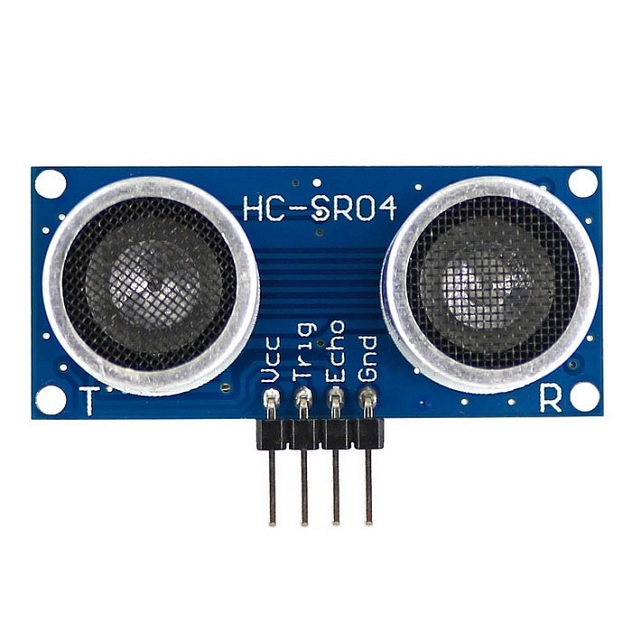
\includegraphics[width=3.5cm]{Figuras/ultrassom.jpg}
    \label{figura:ultrassom.jpeg}
    \end{figure}
    
    \paragraph{}
    O funcionamento do sensor é muito simples, o que muitos podem ter achado se tratar de duas câmeras na verdade são \textbf{um alto-falante e um microfone}. O alto-falante emite uma onda sonora de alta frequência, alta demais para que nós humanos sejamos capazes de escutá-la, essa onda de som é refletida assim que ela vai ao encontro a algum objeto e retorna para o microfone.
    \\~\\
    \textit{Mas qual a utilidade de se emitir um som e depois escutá-lo de volta?} \par
    A funcionalidade não está no som em si, mas sim no \textbf{tempo} que demorou para que a onda sonora retornasse para o sensor, essa informação de tempo é então utilizada para calcular a \textbf{distância do sensor até o objeto} que refletiu a onda de volta.
    
    \paragraph{}
    O sensor ultrassônico é utilizado para obtermos a distância entre o robô e algum objeto à sua frente. Mas nem sempre conseguimos encontrar essa distância como o esperado, isso ocorre pois às vezes o objeto não está bem posicionado, logo, ele não reflete o som de volta para o microfone, ou então ele absorve todo o som, isso pode acontecer se ele for muito macio.
    
    \begin{figure}[h]
    \caption{O objeto tem que se capaz de refletir a onda de volta para o microfone}
     
    \centering 
    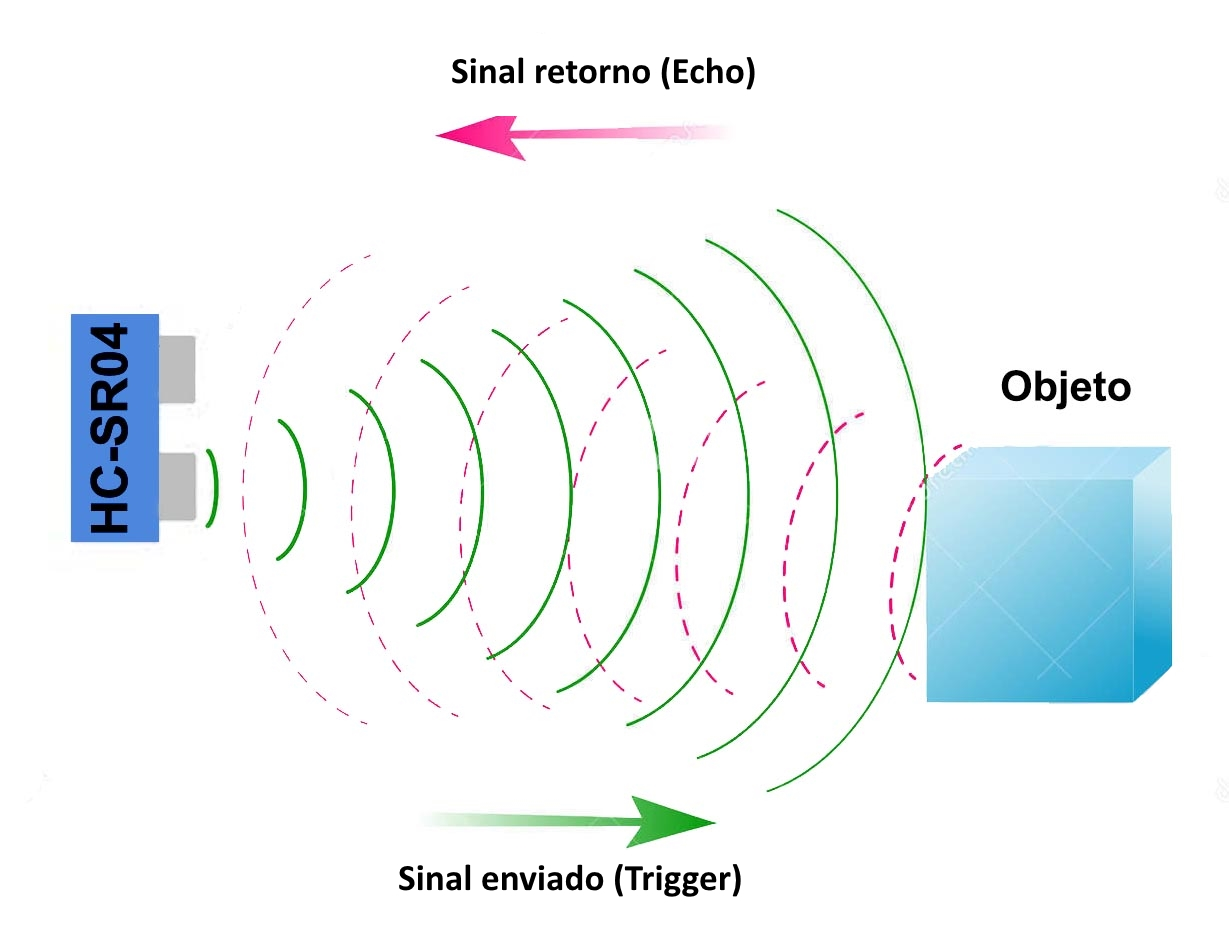
\includegraphics[width=7cm]{Figuras/onda.jpg}
    \label{figura:onda.jpeg}
    \end{figure}
    
\section{Aplicações no Cotidiano}

    \subsection*{Ultrassonografia}
    \paragraph{}
        A Ultrassonografia, também conhecida por Ecografia e Ultrassom, é um exame de diagnóstico que serve para visualizar em tempo real qualquer órgão ou tecido do corpo. Ela é comumente usada para observar o desenvolvimento do feto durante a gravidez. \par 
        Sabe aquelas imagens cinzas borradas que ninguém além do médico é capaz de compreender? Elas são feitas utilizando o ultrassom.
        
    \subsection*{Ecolocalização}
    \paragraph{}
        Embora não seja utilizada por seres humanos, a ecolocalização ou biossonar é muito importante na vida de diversos animais como morcegos, golfinhos e baleias. Eles são seres capazes de emitir ondas de alta frequência e cronometrar o tempo levado até que eles consigam escutar o seu próprio eco, assim, são capazes de conhecer seus arredores mesmo sem o uso da visão.
        
    \subsection*{Sonares}
    \paragraph{}
        Sonares são muito utilizados por navios e submarinos para detectar a presença de outros corpos debaixo da água, seu funcionamento é idêntico ao de um biossonar utilizado por uma baleia, por exemplo. Sonares diferem dos radares pois os radares utilizam ondas de rádio para medir a distância.
        
\section*{Função}

    \paragraph{}
    Para podermos utilizar o sensor ultrassônico presente no \textit{Sparki} tudo o que precisamos fazer é escrever a função \lstinline[columns=fixed]{sparki.ping()} que ela ativará o sensor. Como já dito, o sensor serve para medir a distância, logo, quando o ativamos, espera-se que recebamos algum valor de volta que indique qual é essa distância. Então, função \lstinline[columns=fixed]{sparki.ping()} já faz os cálculos necessários e nos \textbf{retorna} o valor da distância em \textbf{centímetros}.
    \\~\\
    \textit{A função então nos devolve um valor, mas como que eu vejo isso? Onde que ele vai me falar qual a distância que ele mediu? Ele escreve em algum lugar?} \par
    AHA! Acabamos de chegar na parte importante desse capítulo, as funções que retornam valores. O \textit{Sparki} irá escrever o valor que o sensor encontrou no local que a gente determinar para isso, mas claro que isso não quer dizer que podemos simplesmente falar para ele escrever a resposta num papel que ele irá fazer (possível, mas o código para isso seria muito grande). Uma forma interessante de resolver este conflito é a seguinte: nós criamos o local onde ele deve escrever a resposta, mas esse local não pode ser qualquer um, ele tem que ser uma \textbf{variável}. Sempre que criamos uma variável temos que definir também o tipo dela, e como, no nosso caso, estamos trabalhando apenas com centímetros é mais adequado criar uma variável do tipo \textbf{int}, ou seja, que armazena números inteiros.
    
    O código que mostra como fazemos isso está escrito logo abaixo:
    
\begin{lstlisting}[language=C]
#include <Sparki.h>;

int distancia_em_cm;

void setup()
{
}

void loop()
{
    distancia_em_cm = sparki.ping();  
    delay(300);
}
\end{lstlisting}

    Nesse código estamos dizendo que o \textit{Sparki} deve executar a função \lstinline[columns=fixed]{sparki.ping()} e salvar o valor que ela retornar dentro da nossa variável \lstinline[columns=fixed]{distancia_em_cm}. Agora que temos a nossa distância salva dentro de uma variável, podemos trabalhar com ela livremente para fazermos o que quiser, como fazer ele escrever o valor numa folha de papel.
    
    É importante notar a presença da função \lstinline[columns=fixed]{delay()} no código, pois o funcionamento do sensor não é tão rápido quanto a velocidade de processamento do nosso robô, então precisamos dar um pequeno intervalo de tempo para que o sensor possa funcionar sem erros.
    
\section{Servo motor}
    
    \paragraph{}
    Se considerarmos o sensor ultrassônico como sendo a ``cabeça'' do robô, é muito útil que tenhamos também um ``pescoço'' que sirva para movimentarmos a ``cabeça'', então surge a necessidade de um servo motor no \textit{Sparki}, mas afinal o que ele é?
    
    \begin{figure}[h]
    \caption{Imagem de um servo motor}
    
    \centering 
    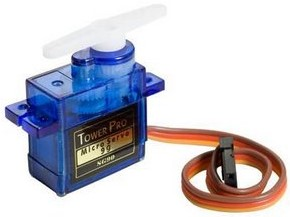
\includegraphics[width=9cm]{Figuras/servo.jpg}
    \label{figura:servo.jpeg}
    \end{figure}

    \paragraph{}
    Um servo motor é um motor que tem a capacidade de girar o seu eixo em ângulos precisos de até 90º ou 180º normalmente, sendo que o servo motor no qual o sensor ultrassônico está acoplado é capaz de girar seu eixo em até 180º. Ele é muito útil para movimentar braços robóticos, por exemplo. Nesse caso não é necessária a realização de voltas completas e a precisão torna-se muito importante. No nosso caso, utilizamos dele para girar o sensor e, assim, podermos medir distâncias em outras direções sem ter que utilizar as rodas para girar o robô, infelizmente não temos como fazer o \textit{Sparki} olhar para cima ou para baixo utilizando um servo motor apenas.
    
\subsection{Função}

    \paragraph{}
    Agora que sabemos da existência do servo motor, precisamos saber como utilizá-lo. Para começar, devemos ativá-lo escrevendo a função \lstinline[columns=fixed]{sparki.servo()}, esta função deve receber um valor de angulação em graus, que determina o quanto ele deve girar, este valor deve estar entre -90º e 90º (sendo valores negativos para a esquerda e positivos para a direita) e o valor pode ser um número quebrado, isto é, o argumento da função é do tipo \textbf{float}.
    
    \paragraph{}
    Para facilitar a nossa vida, a função \lstinline[columns=fixed]{sparki.servo()} já vem com 3 valores predefinidos dos ângulos mais utilizados: SERVO\underline{\hspace{.1in}}LEFT (-90º),  SERVO\underline{\hspace{.1in}}CENTER (0º) e SERVO\underline{\hspace{.1in}}RIGHT (90º), assim tudo o que precisamos fazer é escrever SERVO\underline{\hspace{.1in}}| com o sentido desejado como argumento que o \textit{Sparki} se encarrega de colocar o sensor na posição correta.
    \\~\\
    Abaixo temos um código que faz com que o \textit{Sparki} meça a distância dele para os objetos na sua esquerda, frente, direita e diagonais esquerda e direita.

\begin{lstlisting}[language=C]
#include <Sparki.h>;

int distancia_esquerda, distancia_direita, distancia_frente,
distancia_diagonal_esquerda, distancia_diagonal_direita;

void setup()
{
    sparki.servo(SERVO_LEFT);   //gira para a posição -90 graus
    delay(500)
    distancia_esquerda = sparki.ping();  
    delay(500);
    sparki.servo(-45);   //gira para a posição -45 graus
    delay(500)
    distancia_diagonal_esquerda = sparki.ping();  
    delay(500);
    sparki.servo(SERVO_CENTER);   //gira para a posição 0 graus
    delay(500)
    distancia_frente = sparki.ping();  
    delay(500);
    sparki.servo(45);   //gira para a posição 45 graus
    delay(500)
    distancia_diagonal_direita = sparki.ping();  
    delay(500);
    sparki.servo(SERVO_RIGHT);   //gira para a posição 90 graus
    delay(500)
    distancia_direita = sparki.ping();  
    delay(500);
}

void loop()
{
}
\end{lstlisting}    
    

\section{Exercícios}

    \question{Responda a seguinte pergunta: como podemos encontrar a distância até um objeto utilizando apenas as informações do tempo que a onda de alta frequência demorou para retornar ao sensor e a velocidade dessa mesma onda?}
    
    \begin{center}
        \line(1,0){450}
        \vspace{0.2cm}   
        \line(1,0){450}
        \vspace{0.2cm}   
        \line(1,0){450}
        \vspace{0.2cm} 
        \line(1,0){450}
        \vspace{0.4cm} 
    \end{center}

    \question{Com os conhecimentos adquiridos até agora, escreva um pequeno código que mostre a todo momento na tela LCD a distância do \textit{Sparki} até algum objeto que esteja na sua frente.}

    \begin{center}
        \line(1,0){450}
        \vspace{0.2cm}   
        \line(1,0){450}
        \vspace{0.2cm}   
        \line(1,0){450}
        \vspace{0.2cm}   
        \line(1,0){450}
        \vspace{0.2cm}   
        \line(1,0){450}
        \vspace{0.4cm} 
    \end{center}
    
    \question{Escreva um código que centre o sensor ultrassônico quando o \textit{Sparki} é ligado e que depois de 3 segundos faça ele ficar balançando o sensor de um lado para o outro.}
    
    \begin{center}
        \line(1,0){450}
        \vspace{0.2cm}   
        \line(1,0){450}
        \vspace{0.2cm}   
        \line(1,0){450}
        \vspace{0.2cm}   
        \line(1,0){450}
        \vspace{0.2cm}   
        \line(1,0){450}
        \vspace{0.4cm} 
    \end{center}

    \question{Escreva um código que faça com que o \textit{Sparki} determine a distância até o objeto logo a sua frente e então ande na direção dele e pare a 7cm de distância do objeto.}

    \begin{center}
        \line(1,0){450}
        \vspace{0.2cm}   
        \line(1,0){450}
        \vspace{0.2cm}   
        \line(1,0){450}
        \vspace{0.2cm}   
        \line(1,0){450}
        \vspace{0.2cm}   
        \line(1,0){450}
        \vspace{0.4cm} 
    \end{center}
    
    \challenge{\large{Desafio: Escreva um código onde o \textit{Sparki} gira em até 360º e então mostra na tela LCD as distâncias dos objetos a sua volta nas direções norte, nordeste, leste, sudeste, sul, sudoeste, oeste e noroeste.}}
    
    \begin{center}
        \line(1,0){450}
        \vspace{0.2cm}   
        \line(1,0){450}
        \vspace{0.2cm}   
        \line(1,0){450}
        \vspace{0.2cm}   
        \line(1,0){450}
        \vspace{0.2cm}   
        \line(1,0){450}
        \vspace{0.4cm} 
    \end{center}
\chapter{\textit{If e else}}
\section*{Introdução}
    \paragraph{}
    Neste capítulo aprofundaremos nosso estudo de programação por meio de comandos que permitem a tomada de decisão, ou seja,  estruturas auxiliares que estabelecem uma condição para a execução de um comando principal. \textsl{Ficou confuso? Não se preocupe, vou explicar a seguir!}

\section{Estruturas de decisão}
    \paragraph{}
    Desde o momento em que acordamos, estamos tomando decisões, às vezes até sem perceber! Por exemplo, optar por ficar alguns minutos a mais na cama e adiar o despertador ou decidir levantar no instante em que ele tocar. Vamos supor que amanhã você tem uma prova muito importante às 8 horas da manhã, o fato de escolher ignorar o despertador e dormir mais pode resultar em consequências, como perder aquela prova de final de semestre e, possivelmente, acabar ficando com nota baixa. Como não é isso que queremos, é sempre bom acordar cedo em dias que tivermos provas pela manhã.
    
    Estabelecemos uma condição para acordar cedo, você percebeu? A condição de acordar cedo é se houver uma prova pela manhã... É exatamente isso que faremos neste capítulo! Estabeleceremos condições para que o \textsl{Sparki} realize determinada ação!

\begin{center}
    
   \textcolor{mydarkblue}{\textbf{Para não esquecer!}}
   \\As estruturas de decisão que utilizaremos são ``if'' e ``else'', elas significam ``se'' e ``senão'' em inglês, respectivamente.
    \end{center}
    
    
\section{Como utilizar ``if'' e else''?}
    A seguir temos exemplos de uso dessas estruturas:
    \\~\\
    \textsc{Exemplo 1)} (Apenas para fins didáticos)
\begin{lstlisting}[language=C]
if(Condição 1) 
{
    Ação 1;
} else 
{
    Ação 2;
}
\end{lstlisting}
    
    Esse exemplo significa que, se a ``Condição 1'' for verdadeira, o \textsl{Sparki} executará a ``Ação 1'', senão, ele executará a ``Ação 2''. Utilizar o \lstinline[columns=fixed]{else} como uma opção alternativa ao \lstinline[columns=fixed]{if()} é optativo, ou seja, podem existir expressões condicionais apenas com \lstinline[columns=fixed]{if()}.
    
    \begin{center}
    {\large{Reflita}}: A ``Ação 1'' e a ``Ação 2'' poderiam ser executadas sequencialmente, em apenas uma leitura desse código ?
    \end{center}
    
    A seguir temos uma tabela com todas as opções de execução do código desse primeiro exemplo: (Tente entender a tabela, apenas decorar pode te deixar confuso mais para frente)
    
    \begin{center}
    \begin{tabular}{|c|c|c|}
    \hline
    Condição 1 & Ação 1 & Ação 2 \\ \hline
    Verdadeira & Executa & Não executa \\ \hline
    Falsa & Não executa & Executa \\ \hline
    \end{tabular}
    \end{center}
    
    \textsc{Exemplo 2)} Exemplo da explicação. (Apenas para fins didáticos)
    
\begin{lstlisting}[language=C]
if(For dia de prova) 
{
    Acordar mais cedo;
} else 
{
    Acordar no horário normal;
}
\end{lstlisting}
    
    Neste caso, se for o dia da prova, devemos acordar mais cedo e, se não for o dia da prova, devemos acordar no horário normal. A segunda ação apenas ocorre se a primeira não ocorrer, logo, essas duas ações não poderiam ser executadas sequencialmente, ou seja, em uma mesma verificação da condição de ser ou não dia de prova.

    \textsc{Exemplo 3)} Exemplo com ``else if''. (Apenas para fins didáticos)
    \begin{lstlisting}[language=C]
if(Condição 1)
{
    Ação 1;
} else if(Condição 2)
{
    Ação 2;
} else
{
    Ação 3;
}
\end{lstlisting}
    
    \textit{Agora apareceram \lstinline[columns=fixed]{else} e \lstinline[columns=fixed]{if} em uma mesma linha, o que isso significa?} \par
    Para entender os dois termos juntos, vamos revisar o significado deles separados. \lstinline[columns=fixed]{else} significa: ``se as condições anteriores forem falsas, executar o comando dentro das chaves''. \lstinline[columns=fixed]{if()} significa: ``se a condição dentro dos parênteses for verdadeira, executar o comando dentro das chaves''. Consequentemente, a expressão \lstinline[columns=fixed]{else if()} implica na execução do comando apenas se as condições anteriores forem falsas e a condição dentro do parênteses for verdadeira.
    
    \begin{center}
    \begin{tabular}{|c|c|c|c|c|}
    \hline
    Condição 1 & Ação 1 & Condição 2 & Ação 2 & Ação 3\\ \hline
    Verdadeira & Executa & Falsa & Não executa & Não executa \\ \hline
    Verdadeira & Executa & Verdadeira & Não executa & Não executa \\ \hline
    Falsa & Não executa & Verdadeira & Executa & Não executa \\ \hline
    Falsa & Não executa & Falsa & Não executa & Executa \\ \hline
    \end{tabular}
    \end{center}
    
    \textsc{Exemplo 4)} Imagine uma situação hipotética em que existam 3 compromissos na sua agenda, no mesmo dia e horário, e você terá que escolher apenas um, de acordo com a previsão do tempo. (Apenas para fins didáticos)
    
    \begin{lstlisting}[language=C]
if(Estiver fazendo muito calor)
{
    Ir ao clube;
} else if(Estiver chovendo)
{
    Ver um filme em casa;
} else if(Estiver nevando)
{
    Ir esquiar;
} else
{
    Ir ao cinema;
}
\end{lstlisting}
    
    \textit{Isshh... Agora ficou complicado! E se a previsão do tempo afirmar que vai chover e nevar nesse dia? Qual compromisso eu escolho?} \par
    Essa é fácil! É necessário apenas observar qual das condições será lida primeiro nesse código, ou seja, o que vier primeiro! Como a condição ``Estiver chovendo'' aparece primeiro, o compromisso seria ``Ver um filme em casa''. \\

    \textit{E qual seria a condição para ``Ir ao cinema''?} \par
    A condição seria a negação das anteriores, neste caso, se não estivesse fazendo muito calor, nem chovendo, nem nevando.
    
    \paragraph{}
    Uma curiosidade dessa estrutura condicional é que se escrevermos 1 dentro dos parênteses do \lstinline[columns=fixed]{if()}, ele será verdadeiro e o que estiver dentro das chaves será executado. Assim, se escrevermos 0 dentro dos parênteses, o \lstinline[columns=fixed]{if()} será falso e o que estiver dentro das chaves não será executado. Isso se dá porque a programação possui uma base binária, ou seja, ela é baseada em vários 1's e 0's, sendo 1 verdadeiro e 0 falso.
    
    \section{Operações de comparação}
    
    \paragraph{}
    Iremos aprender nesta seção os tipos de operadores que podemos utilizar para comparar dois valores ou incógnitas. Lembrando que eles devem ser utilizados apenas dentro do parênteses do \lstinline[columns=fixed]{if()}. São eles:
    
    \begin{itemize}
        \item \lstinline[columns=fixed]{==} para verificar se os dois valores são iguais.
        \item \lstinline[columns=fixed]{!=} para verificar se os dois valores são diferentes.
        \item \lstinline[columns=fixed]{>} para verificar se o primeiro é maior que o segundo.
        \item \lstinline[columns=fixed]{>=} para verificar se o primeiro é maior que o segundo ou igual a ele.
        \item \lstinline[columns=fixed]{<} para verificar se o primeiro é menor que o segundo.
        \item \lstinline[columns=fixed]{<=} para verificar se o primeiro é menor que o segundo ou igual a ele.
    \end{itemize}
    
    Agora que você já entendeu como funcionam as expressões condicionais e os operadores de comparação, vamos para um exemplo de verdade!
    \\~\\
    \textsc{Exemplo 1)} Atribuiremos o valor 2042385 à variável x e queremos que o \textsl{Sparki} responda se esse número é ímpar ou par. Para isso, utilizaremos a informação da sessão anterior sobre os 1's e os 0's.

    \begin{lstlisting}[language=C]
#include <Sparki.h>;

void setup()
{
}

void loop()
{
    int x = 2042385;
    sparki.clearLCD();
    if(x % 2) 
    {
        sparki.print("O numero e impar.");
    } else 
    {
        sparki.print("O numero e par.");
    }
    sparki.updateLCD();
    delay(1000);
}
\end{lstlisting}
    
    Sabemos que o número 2042385 é ímpar pela regra da divisão por 2, que afirma que um número é divisível por 2 quando o último algarismo dele for divisível por 2. Nesse código, não utilizamos essa regrinha, mas sim o método mais tradicional, fazemos o \textsl{Sparki} verificar se a divisão desse número por 2 é exata, ou seja, se o resto é 0. Assim, o \textsl{Sparki} chega a mesma conclusão que chegamos, que o número 2042381 é ímpar, e imprime essa informação no LCD.
    
    \begin{center}
    \textcolor{mydarkblue!80!black}{\textbf{Lembrando:}}
    O símbolo ``\%'' significa o resto da divisão do primeiro número pelo segundo.
    \\ Exemplo:
    $10\%2 = 0$ e $10\%3 = 1$
    \end{center}
    
    \textsc{Exemplo 2)} Dessa vez, faremos com que o \textsl{Sparki} responda se o número 2042385 é divisível por 3 e por 5.
    
    \begin{lstlisting}[language=C]
#include <Sparki.h>;

void setup()
{
}

void loop()
{
    int x = 2042385;
    sparki.clearLCD();
    if((x % 3) == 0) 
    {
        sparki.println("O numero e divisivel por 3.");
    } else 
    {
        sparki.println("O numero nao e divisivel por 3.");
    }
    if((x % 5) == 0) 
    {
        sparki.print("O numero e divisivel por 5.");
    } else 
    {
        sparki.print("O numero nao e divisivel por 5.");
    }
    sparki.updateLCD();
    delay(1000);
}
\end{lstlisting}

    
    Esse exemplo é parecido com o anterior, mas ele está aqui para mostrar que podemos inserir duas estruturas condicionais independentes em um mesmo código. As duas comparações para saber se o número é divisível por 3 e por 5 não dependem uma da outra, pois um número pode ser divisível por 3 e por 5 ao mesmo tempo, por isso que existem dois \lstinline[columns=fixed]{if()} e dois \lstinline[columns=fixed]{else}. Consequentemente, o \textsl{Sparki} imprimirá duas mensagens na tela, na primeira linha: ``O numero e divisivel por 3'' e na segunda: ``O numero e divisivel por 5''.
    
    \textsc{Exemplo 3)} Exemplo de comparação de variáveis.
    
    \begin{lstlisting}[language=C]
#include <Sparki.h>;

void setup()
{
}

void loop()
{
    int x = 10;
    int y = 100;
    sparki.clearLCD();
    if(x >= y) {
        sparki.print("Condicao 1");
    } else if(y != (x * x)) {
        sparki.print("Condicao 2");
    } else if((y / x) >= x) {
        sparki.print("Condicao 3");
    } else if((y - 100) <= x){
        sparki.print("Condicao 4");
    }
    sparki.updateLCD();
    delay(1000);
}
\end{lstlisting}

    Você reparou que a disposição das chaves no código está diferente das utilizadas anteriormente? Os dois modos são válidos, sendo as chaves coladas no if ou em outra linha, mas é sempre bom manter um padrão, por isso, antes de começar um código, decida qual será a convenção utilizada. Então, já sabe o que o \textsl{Sparki} fará ao ler este código? Vamos ver passo a passo:
    
    \begin{itemize}
        \item[Condição 1)]
        \begin{eqnarray}
        x & >= & y\\
        10 & >= & 100 \nonumber     \end{eqnarray}
        Essa afirmação é FALSA, logo, o \textsl{Sparki} não executará a ação entre as chaves.
        \item[Condição 2)]
        \begin{eqnarray}
        y & != & (x * x)\\
        100 & != & 10 * 10 \nonumber\\
        100 & != & 100 \nonumber
        \end{eqnarray}
        Essa afirmação também é FALSA, por isso a ação não será executada.
        \item[Condição 3)]
        \begin{eqnarray}
        (y / x) & >= & x\\
        (100 / 10) & >= & 10 \nonumber\\
        10 & >= & 10 \nonumber\\
        \end{eqnarray}
        Essa afirmação é verdadeira, logo, o \textsl{Sparki} executará a ação entre as chaves, imprimirá no LCD ``Condicao 3''.
        \item[Condição 4)]
        Essa condição não será nem lida, pois ela só poderia ser executada se todos os \lstinline[columns=fixed]{if()} anteriores, dentro dessa estrutura condicional, fossem falsos.
    \end{itemize}
    
    \begin{center}
    \textcolor{teal}{Lembrando:}
    Sempre devemos executar a operação dentro dos parênteses antes dos operadores de comparação. 
    \end{center}
 
\section{Operadores lógicos}
    \paragraph{}
    Nesta seção, iremos aprender a lidar com comparações que envolvem mais de um fator a ser analisado e, para isso, utilizaremos o início da teoria da Álgebra Booleana, criada por George Boole. Na Álgebra de Boole, existem 3 tipos de operadores lógicos: E, OU e NÃO, cada um com uma funcionalidade própria. Eles devem ser usados dentro de condicionais \lstinline[columns=fixed]{if()} para ligar duas comparações ou para negar uma ou mais comparações.
 
\subsection{E (AND)}
 
    \paragraph{}
    Este operador depende de pelo menos dois ``resultados'' de afirmações, por exemplo, vamos supor que você quer ir à piscina, mas você apenas irá se estiver fazendo sol E se a piscina estiver limpa. Então, a 1ª afirmação é: se estiver fazendo sol e a 2ª afirmação é: se a piscina estiver limpa. O operador AND vai funcionar como uma ``ponte'' de ligação entre essas duas afirmações. 
    
    \begin{center}
        A condição estabelecida pelo \lstinline[columns=fixed]{if()}, com o AND entre as afirmações, será VERDADEIRA apenas quando as afirmações forem ambas VERDADEIRAS.
    \end{center}
    
    \textit{Então o AND vai ser uma comparação entre duas comparações?? Que confuso!} \par
    Mais ou menos... É mais certo dizer que o AND irá realizar uma operação entre as duas comparações/afirmações. Utilizando o exemplo anterior, as duas afirmações têm que ser verdadeiras, ou seja, 1) tem que estar fazendo sol e 2) a piscina tem que estar limpa para que a comparação seja verdadeira e você possa ir à piscina.
    \\~\\
    \textsc{Exemplo 0)} Exemplo da explicação, apenas para fins didáticos.
    \begin{lstlisting}[language=C]
if(Fizer sol AND Piscina estiver limpa)
{
    Ir à piscina;
} else 
{
    Não ir à piscina;
}
\end{lstlisting}

    Se a comparação 1 der VERDADEIRA e a comparação 2 der FALSA, o \lstinline[columns=fixed]{if()} não será realizado e você não irá à piscina. Porém, se as duas comparações derem VERDADEIRAS, o \lstinline[columns=fixed]{if()} será realizado e você poderá ir à piscina.
    
    Agora, vamos fazer um esquema com todas as possibilidades de combinação entre duas comparações e ver o resultado final:
    
    \begin{itemize}
        \item VERDADEIRO AND VERDADEIRO -> Resultado: VERDADEIRO
        \item VERDADEIRO AND FALSO -> Resultado: FALSO
        \item FALSO AND VERDADEIRO -> Resultado: FALSO
        \item FALSO AND FALSO -> Resultado: FALSO
    \end{itemize}
    
    \begin{center}
    \textcolor{mydarkblue!80!black}{\textbf{Lembrando:}}
    Resultado: VERDADEIRO, significa que o \lstinline[columns=fixed]{if()} será executado. 
    Resultado: FALSO, significa que o \lstinline[columns=fixed]{if()} não será executado.
    \end{center}
 
    \textit{Tá, mas como eu aplico isso na programação?}
        
    Na programação, utilizamos os caracteres \lstinline[columns=fixed]{&&} para simbolizar o AND. 
    Aqui temos um exemplo:
    \\~\\
    \textsc{Exemplo 1)} Neste exemplo, serão criadas 3 variáveis para armazenar a idade de 3 crianças: o Enzo, que tem 1 ano, a Valentina, que tem 2 anos, e a Sofia com 3 anos. Se a idade das 3 crianças forem iguais, o \textsl{Sparki} andará para frente, se a Sofia for a mais velha e o Enzo o mais novo, o \textsl{Sparki} andará para trás, e, por último, se as duas condições anteriores forem falsas, o \textsl{Sparki} ficará parado.

    \begin{lstlisting}[language=C]
#include <Sparki.h>;

void setup()
{
}

void loop()
{
    int idade_enzo = 1;
    int idade_valentina = 2;
    int idade_sofia = 3;
    if(idade_enzo == idade_valentina && idade_enzo == idade_sofia){
        //Se o Enzo e a Valentina e a Sofia tiverem a mesma idade
        //Neste caso, FALSO AND FALSO -> Resultado: FALSO
        sparki.moveForward();
    } else if(idade_valentina > idade_enzo && idade_sofia > idade_valentina) 
    {
        //Se o primeiro caso "if" for falso e a Sofia for mais velha que a 
        //Valentina, que for mais velha que o Enzo
        //Neste caso, VERDADEIRO AND VERDADEIRO -> Resultado: VERDADEIRO
        sparki.moveBackward();
    } else 
    {
        //Se o primeiro e o segundo caso forem falsos
    }
}
\end{lstlisting}

    
    O \textsl{Sparki} andará para trás.
    \begin{itemize}
        \item[Condição 1)]
        \begin{eqnarray}
        idade\_enzo & = & idade\_valentina\\
        1 & = & 2 \nonumber     \end{eqnarray}
        Essa afirmação é FALSA.
        \begin{eqnarray}
        idade\_enzo & == & idade\_sofia\\
        1 & == & 3 \nonumber
        \end{eqnarray}
        Essa afirmação é FALSA.
        Como temos o \lstinline[columns=fixed]{&&} (AND) ligando as duas afirmações, a comparação será FALSA.
        \item[Condição 2)]
        \begin{eqnarray}
        idade\_valentina & > & idade\_enzo
        \end{eqnarray}
        Essa afirmação é VERDADEIRA.
        \begin{eqnarray}
        idade\_sofia & > & idade\_valentina
        \end{eqnarray}
        Essa afirmação também é VERDADEIRA. Como as duas afirmações são verdadeiras e o \lstinline[columns=fixed]{&&} (AND) está ligando-as, a comparação será VERDADEIRA.
    \end{itemize} 
    
    \textsc{Exemplo 2)} Um exemplo com as mesmas variáveis anteriores, mas um pouco mais complicado.
    
    \begin{lstlisting}[language=C]
#include <Sparki.h>;

void setup()
{
}

void loop()
{
    int idade_enzo = 1;
    int idade_valentina = 2;
    int idade_sofia = 3;
    sparki.clearLCD();
    if((idade_sofia - idade_valentina) == idade_enzo &&
        (idade_valentina - idade_enzo) == 3) 
    {
        //VERDADEIRO AND FALSO -> Resultado: FALSO
        sparki.drawCircleFilled(63, 32, 10);
    } else if((idade_enzo + 1) != 2 && (idade_valentina - idade_enzo) != idade_sofia) 
    {
        //FALSO AND VERDADEIRO -> Resultado: FALSO
        sparki.drawRectFilled(10,0, 15, 30);
    } else if((idade_enzo * 6) == (idade_valentina * 3)) 
    {
        //VERDADEIRO
        sparki.drawChar(10, 1, 'a');
    } else 
    {
        sparki.drawString(40, 4, "123");
    } 
    sparki.updateLCD();
    delay(1000);
}
\end{lstlisting}

    
    O \textsl{Sparki} irá imprimir o caracter ``a'' no LCD.
    \begin{itemize}
        \item[Condição 1)]
        \begin{eqnarray}
        (idade\_sofia - idade\_valentina) & = & idade\_enzo\\
        (3 - 2) & = & 1 \nonumber \\
        1 & = & 1 \nonumber
        \end{eqnarray}
        Essa afirmação é VERDADEIRA.
        \begin{eqnarray}
        (idade\_valentina - idade\_enzo) & = & 3\\
        (2 - 1) & = & 3 \nonumber \\
        1 & = & 3 \nonumber
        \end{eqnarray}
        Essa afirmação é FALSA.
        Como temos o ``\&\&'' (AND) ligando essas duas afirmações, a comparação será FALSA.
        \item[Condição 2)] 
        \begin{eqnarray}
        (idade\_enzo + 1) & != & 2\\
        (1 + 1) & != & 2 \nonumber \\
        2 & != & 2 \nonumber
        \end{eqnarray}
        Essa afirmação é FALSA.
        \begin{eqnarray}
        (idade\_valentina - idade\_enzo) & != & idade\_sofia)\\
        (2 - 1) & != & 3 \nonumber \\
        1 & != & 3 \nonumber
        \end{eqnarray}
        Essa afirmação é VERDADEIRA. Como o \lstinline[columns=fixed]{&&} (AND) está ligando essas duas afirmações, a comparação será FALSA
        \item[Condição 3)] 
        \begin{eqnarray}
        (idade\_enzo * 6) & = & (idade\_valentina * 3)\\
        (1 * 6) & = & (2 * 3) \nonumber \\
        6 & = & 6 \nonumber 
        \end{eqnarray}
        Essa afirmação é VERDADEIRA, logo, a comparação também é.
    \end{itemize}
    
    \begin{center}
    \textcolor{mydarkblue}{\textbf{Para não esquecer!}}
    \\``And'' traduzido para o português significa ``e''.
    \end{center}
     
\subsection{OU (OR)}
    \paragraph{}
    Este operador deve ser colocado entre duas ou mais afirmações, assim como o AND. Vamos supor que a sua mãe está viajando e você combinou de se encontrar com ela quando ela chegasse no aeroporto. O combinado foi o seguinte: ela mandaria mensagem \textbf{OU} ligaria quando estivesse embarcando no voo de volta, e você sairia de casa por volta de 30 minutos depois, para se encontrar com ela no aeroporto.
    
    \begin{center}
        A condição estabelecida pelo \lstinline[columns=fixed]{if()}, com o OR entre as afirmações, será VERDADEIRA se pelo menos uma das duas comparações forem VERDADEIRAS.
    \end{center}
   
    \textsc{Exemplo 0)} Exemplo da explicação, apenas para fins didáticos.
    \begin{lstlisting}[language=C]
if(Sua mãe te mandasse mensagem OR Sua mãe te ligasse)
{
    Esperar 30 minutos;
    Sair de casa;
} else
{
    Continuar esperando a mensagem ou a ligação;
}
\end{lstlisting}

    Então, se a sua mãe te ligasse (afirmação VERDADEIRA) mas não te mandasse mensagem (afirmação FALSA), a condição do \lstinline[columns=fixed]{if()} seria VERDADEIRA e você esperaria 30 minutos para sair de casa. Se as duas afirmações foram VERDADEIRAS, ou seja, se ela te mandar mensagem e te ligar, a condição \lstinline[columns=fixed]{if()} também será VERDADEIRA, neste caso, você também executará as ações dentro das chaves do \lstinline[columns=fixed]{if()}.
     A seguir temos todos os resultados possíveis para um OR entre duas afirmações:
     
     \begin{itemize}
        \item VERDADEIRO OR VERDADEIRO -> Resultado: VERDADEIRO
        \item VERDADEIRO OR FALSO -> Resultado: VERDADEIRO
        \item FALSO OR VERDADEIRO -> Resultado: VERDADEIRO
        \item FALSO OR FALSO -> Resultado: FALSO
    \end{itemize}
    
    Na programação, utilizamos os caracteres \lstinline[columns=fixed]{||} para simbolizar o OR.
    \\~\\
    \textsc{Exemplo 1)}
     
    \begin{lstlisting}[language=C]
#include <Sparki.h>;

void setup()
{
}

void loop()
{
    int idade_enzo = 1;
    int idade_valentina = 2;
    int idade_sofia = 3;
    if(idade_enzo == idade_valentina || idade_sofia != idade_ valentina) 
    {
        //Neste caso, FALSO OR VERDADEIRO -> Resultado: VERDADEIRO
        sparki.moveBackward();
    } else if(idade_valentina ==  (idade_sofia - 1) ||
             (idade_valentina + 1) == idade_sofia) 
    {
        //Neste caso, VERDADEIRO OR VERDADEIRO -> Resultado: VERDADEIRO
        sparki.moveForward();
    } else 
    {
        //Se a primeira e a segunda condição forem falsas
        sparki.moveRight();
    }
}
\end{lstlisting}

    
    O \textsl{Sparki} andará para trás.
    \begin{itemize}
        \item[Condição 1)] 
        \begin{eqnarray}
        idade\_enzo & = & idade\_valentina
        \end{eqnarray}
        Essa afirmação é FALSA.
        \begin{eqnarray}
        idade\_sofia & != & idade\_valentina
        \end{eqnarray}
        Essa afirmação é VERDADEIRA. Como o \lstinline[columns=fixed]{||} (OR) liga essas duas afirmações, sabemos que a comparação será VERDADEIRA.
        \item[Condição 2)] Essa condição não será nem lida, pois ela só poderia ser executada se todos os \lstinline[columns=fixed]{if()} anteriores, dentro dessa estrutura condicional, fossem falsos.
    \end{itemize}

    \textsc{Exemplo 2)}
     
    \begin{lstlisting}[language=C]
#include <Sparki.h>;

void setup()
{
}

void loop()
{
    int idade_enzo = 1;
    int idade_valentina = 2;
    int idade_sofia = 3;
    sparki.clearLCD();
    if(idade_valentina != 2 || idade_enzo != 1) 
    {
        //FALSO OR FALSO -> Resultado: FALSO
        sparki.print("Condicao 1");
    } else if(idade_sofia != (idade_valentina - 1) && idade_sofia == idade_enzo) 
    {
        //VERDADEIRO AND FALSO -> Resultado: FALSO
        sparki.print("Condicao 2");
    } else if((idade_enzo + 2) == (idade_sofia + 1) ||
              idade_enzo == (4 - idade_sofia)) 
    {
        //FALSO OR VERDADEIRO -> Resultado: VERDADEIRO
        sparki.print("Condicao 3");
    } else 
    {
        sparki.print("Nenhuma das anteriores");
    }
    sparki.updateLCD();
    delay(1000);
}
\end{lstlisting}
    
    O \textsl{Sparki} irá imprimir na tela ``Condição 3''.
    \begin{itemize}
        \item[Condição 1)] 
        \begin{eqnarray}
        idade\_valentina != 2\\
        idade\_enzo != 1 \nonumber
        \end{eqnarray}
        Ambas afirmações são FALSAS.
        \item[Condição 2)]
        \begin{eqnarray}
        idade\_sofia & = & idade\_enzo;
        \end{eqnarray}
        Essa afirmação é FALSA.
        \item[Condição 3)]
        \begin{eqnarray}
        (idade\_enzo + 2) & = & (idade\_sofia + 1)\\
        (1 + 2) & = & (3 + 1) \nonumber \\
        3 & = & 4 \nonumber
        \end{eqnarray}
        Essa afirmação é FALSA;
        \begin{eqnarray}
        idade\_enzo & = & (4 - idade\_sofia)\\
        1 & = & 4 - 3 \nonumber \\
        1 & = & 1 \nonumber
        \end{eqnarray}
        Essa afirmação é VERDADERIA, logo FALSO OR VERDADEIRO -> Resultado: VERDADEIRO.
    \end{itemize}
     
    \begin{center}
        \textcolor{mydarkblue}{\textbf{Para não esquecer!}}
        \\``Or'' traduzido para o português significa ``ou''.
    \end{center}
     
\subsection{NÃO (NOT)}

    \begin{itemize}
        \item NOT(VERDADEIRO) -> Resultado: FALSO
        \item NOT(FALSO) -> Resultado: VERDADEIRO
    \end{itemize}
    
    Na programação, utilizamos o caracter \lstinline[columns=fixed]{!} para simbolizar o NOT.
    \\~\\
    \textsc{Exemplo 1)}
     
    \begin{lstlisting}[language=C]
#include <Sparki.h>;

void setup()
{
}

void loop()
{
    int idade_enzo = 1;
    int idade_valentina = 2;
    int idade_sofia = 3;
    if(!(idade_enzo == 1) 
    {
        //NOT(VERDADEIRO) -> Resultado: FALSO
    } else if(!(idade_valentina == 3)) 
    {
        //NOT(FALSO) -> Resultado: VERDADEIRO
        sparki.moveForward();
    } else if(!(idade_sofia != 3)) 
    {
        //NOT(FALSO) -> Resultado: VERDADEIRO
        sparki.moveBackward();
    }
}
\end{lstlisting}

    O \textsl{Sparki} andará para frente, pois
    \begin{itemize}
        \item[Condição 1)]
        \begin{eqnarray}
        !(idade\_enzo & = & 1)\\
        !(1 & = & 1) \nonumber         \end{eqnarray}
        Sabemos que a afirmação 1 = 1 é VERDADEIRA, mas há um caracter \lstinline[columns=fixed]{!} antes dela, por isso, ela acaba se tornando FALSA.
        \item[Condição 2)]
        \begin{eqnarray}
        !(idade\_valentina & = & 3)\\
        !(2 & = & 3) \nonumber
        \end{eqnarray}
        A afirmação 2 = 3 é FALSA, mas o caracter \lstinline[columns=fixed]{!} antes dela a torna VERDADEIRA.
        \item[Condição 3)] Essa condição não será lida.
    \end{itemize}
    
    \begin{center}
        \textcolor{mydarkblue}{\textbf{Para não esquecer!}}
        \\``Not'' traduzido para o português significa ``não''.
    \end{center}

\section{LCD2: fazendo uma animação na tela do Sparki}

    \paragraph{}
    Agora que aprendemos o que são variáveis e estruturas de condição, podemos fazer uma animação. Mas como ainda somos iniciantes na programação, iremos começar a movimentar um objeto bem simples e conhecido na tela do \textsl{Sparki}, um círculo.\par
    Para fazer essa animação, siga os seguintes passos e vamos nessa!
    
    \begin{lstlisting}[language=C]
#include <Sparki.h>;

void setup()
{
}

void loop()
{
    int x = 0;
    sparki.clearLCD();
    if (x < 127) 
    {
        x++;
    }
    else
    {
      x = 0;
    }
    sparki.drawCircleFilled(x, 32, 10);
    sparki.updateLCD();
    delay(100);
}
\end{lstlisting}

    A ideia desse código é criar círculos com o parâmetro \lstinline[columns=fixed]{x} variando, ou seja, modificando a localização desse círculo cada vez que o \lstinline[columns=fixed]{void loop()} é executado.
    \\~\\
    \textit{Não entendi essa condição de \lstinline[columns=fixed]{x < 127}, o que isso significa?} \par
    Você se lembra de quando vimos no capítulo de LCD que as dimensões da tela do \textit{Sparki} são 127x63 pixels? Significa que ele tem 127 pixels no eixo x (horizontal) e 63 pixels no eixo y (vertical). Então, para ``movimentar'' o círculo para a direita na tela, devemos ir aumentando o valor do \lstinline[columns=fixed]{x} (o valor horizontal), assim, criando novos círculos com os valores atualizados de \lstinline[columns=fixed]{x} e apagando os círculos com o valor de \lstinline[columns=fixed]{x} desatualizado. Isso explica o \lstinline[columns=fixed]{x++}. Agora, voltando para a condição \lstinline[columns=fixed]{x < 127}, como a tela tem 127 pixels de comprimento, se o \lstinline[columns=fixed]{x} assumir valores maiores que 127 ou iguais a 127, o círculo irá ``sumir'' da tela LCD, por isso, criamos essa condição \lstinline[columns=fixed]{else} de \lstinline[columns=fixed]{x = 0} caso \lstinline[columns=fixed]{x >= 127}, para que, caso o círculo chegue ao final da tela, ele seja recriado no início da tela, na próxima sequência do \lstinline[columns=fixed]{void loop()}.
    
\section{Exercícios}

\question{Analise e descubra qual o valor final de x e de y. Além disso, escreva o resultado lógico (verdadeiro ou falso) da comparação de variáveis x == y a partir dos valores finais.}

    \begin{lstlisting}[language=C]
    ...
    int x = 1;
    int y = 0;
    y = x;
    x += 1;
    ...
    \end{lstlisting}

    \begin{center}
        \line(1,0){450}
        \vspace{0.4cm} 
    \end{center}

\question{Caso você tenha que julgar duas condições verdadeiras separadas por um operador OR, qual seria o resultado lógico? E se o operador utilizado fosse AND?}

    \begin{center}
        \line(1,0){450}
        \vspace{0.2cm}   
        \line(1,0){450}
        \vspace{0.4cm} 
    \end{center}

    \question{Qual seria o resultado lógico da seguinte linha de código? Verdadeiro ou falso?}

    \begin{lstlisting}[language=C]
 ...
 ((2 + 3) == 5 || (5) == 5) && ( (3 == 3) && (3 - 1 == 1 + 1))
 ...
\end{lstlisting}

    \begin{center}
        \line(1,0){450}
        \vspace{0.4cm} 
    \end{center}
 
    \question{Leia o seguinte código e marque a alternativa correspondente:}

    \begin{lstlisting}[language=C]
#include <Sparki.h>;

void setup()
{
}

void loop()
{
    a = 5
    b = 10
    c = a + b
    sparki.clearLCD();
    if(a != (b - 5)) 
    {
        sparki.print("Hello World");
    } else if(a == (c - b) && b != (c - a)) 
    {
        sparki.print("Hello");
        sparki.print("World");
    } else if(((a + 5) >= (b + 1)) || (((b + a) == c) && ((b / 2) == a))) 
    {
        sparki.println("Hello");
        sparki.print("World");
    }
    sparki.updateLCD();
    delay(3000);
}
\end{lstlisting}
    
    O que aparecerá na tela LCD do \textsl{Sparki} após 3 segundos?

    \begin{description}
    \item[a)] ``HelloWorld'' em uma linha.
    \item[b)] ``Hello'' em uma linha e ``World'' na linha de baixo.
    \item[c)] ``Hello World'' em uma linha.
    \item[d)] Nenhuma das anteriores.
    \end{description}

    \question{Refaça o código do exemplo 1) da seção de ``Operações de comparação'' utilizando o operador lógico NOT.}

    \begin{center}
        \line(1,0){450}
        \vspace{0.2cm}   
        \line(1,0){450}
        \vspace{0.2cm}   
        \line(1,0){450}
        \vspace{0.2cm}   
        \line(1,0){450}
        \vspace{0.2cm}   
        \line(1,0){450}
        \vspace{0.4cm} 
    \end{center}
    
    \question{Escreva um código para verificar se o número 34534 é divisível por 2 e 3. Se for, imprimir no LCD a mensagem ``Numero divisível por 2 e por 3'', se não for, verificar se este número é divisível por 2 e por 3 isoladamente, com duas estruturas condicionais independentes. Se for divisível apenas por 2, imprimir no LCD ``Numero divisível por 2'', se for divisível apenas por 3, imprimir no LCD ``Numero divisível por 3''.}

    \begin{center}
        \line(1,0){450}
        \vspace{0.2cm}   
        \line(1,0){450}
        \vspace{0.2cm}   
        \line(1,0){450}
        \vspace{0.2cm}   
        \line(1,0){450}
        \vspace{0.2cm}   
        \line(1,0){450}
        \vspace{0.4cm} 
    \end{center}
    
    \challenge{\large{Desafio:} Escreva o que aparecerá na tela do \textsl{Sparki} após 2 segundos.}
    
    \begin{lstlisting}[language=C]
#include <Sparki.h>;

void setup()
{
}

void loop()
{
    int x = 0;
    int y = 10;
    int z = 4;
    sparki.clearLCD();
    y = -2;
    x = y;
    if(!(x == -2)) 
    {
        sparki.print("A"); 
    } else if(y >= -3 && x == y) 
    {
        z = 3;
        x = 1;
        sparki.print("b");
    } else if(z == 3 || x != -2) 
    {
        z = 4;
       sparki.print("c"); 
    }
    sparki.print("D");
    x += 0;
    if(!(x == 0 || z != 3)) 
    {
        sparki.print("E");
        sparki.print("f");
        sparki.updateLCD();
    } else 
    {
        sparki.print("G");
    }
    sparki.updateLCD();
    sparki.print("h");
    delay(2000);
}
\end{lstlisting}

    
    \begin{center}
        \line(1,0){450}
        \vspace{0.2cm} 
        \line(1,0){450}
        \vspace{0.4cm} 
    \end{center}
    
\chapter{Infravermelho}

\section*{Introdução}

\paragraph{}
No capítulo de infravermelho, iremos falar sobre o funcionamento e utilidade que os sensores infravermelhos do \textit{Sparki} possuem. As ondas infravermelhas estão mais presentes no nosso dia a dia do que você pode imaginar, na maioria das vezes elas são úteis quando utilizados receptores de luz infravermelha. Nesse capítulo iremos explicar como que o \textit{Sparki} pode ser controlado pelo controle remoto e como fazê-lo seguir linhas utilizando dessas ondas.

\section{Ondas Infravermelhas}
\paragraph{}
Para começar, que tal falarmos do que exatamente é uma onda infravermelha? Ela, assim como a luz visível, é uma onda eletromagnética, uma onda capaz de se propagar no vácuo. A luz infravermelha é invisível aos olhos humanos, isso porque nossos foto-receptores dentro dos nossos olhos, são incapazes de serem estimulados pela frequência das ondas infravermelhas.
\paragraph{}
Chamamos essa onda de infravermelho, porque a sua frequência é menor do que a frequência da cor vermelha (o prefixo infra indica que algo é inferior). A cor vermelha é a cor com a frequência mais baixa que o ser humano é capaz de enxergar, logo se temos uma onda com frequência menor, ela se torna invisível.

    \begin{figure}[h]
    \caption{Espectro da luz visível}
     
    \centering 
    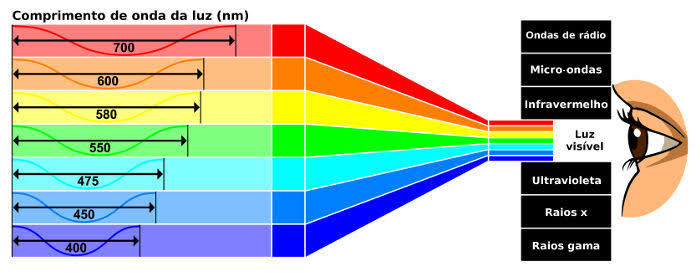
\includegraphics[width=14cm]{Figuras/espectro.jpg}
    \label{figura:espectro.jpeg}
    \end{figure}

\paragraph{}
Você deve estar lembrando do Capítulo de Ultrassom, onde falamos que ondas ultrassônicas são ondas sonoras que os seres humanos são incapazes de escutar porque possuem uma frequência muito alta, essa é a mesma lógica da luz ultravioleta, presente acima na imagem \ref{figura:espectro.jpeg}, elas são ondas eletromagnéticas com frequência mais alta do que a cor violeta, que é a cor com frequência mais alta que nós somos capazes de enxergar, logo ela também é invisível aos nossos olhos. Alguns animais são capazes de ver essas cores, logo eles conseguem ver o mundo ainda mais colorido do que nós humanos.
\paragraph{}
Os raios infravermelhos originam-se dos corpos quentes como o Sol e o corpo de seres vivos por exemplo, cada cor está relacionada com uma temperatura (se você iluminar um termômetro com luzes de cores diferentes, ele irá dar temperaturas diferentes), e o vermelho é a cor mais quente, logo mesmo sem conseguir vermos o infravermelho, ainda somos capazes de sentí-lo porque ele aquece a nossa pele.
\paragraph{}
Esse tipo de onda é muito importante para a vida na Terra, ela é responsável pelo \textbf{efeito estufa}, onde parte dos raios solares ficam presos dentro da nossa atmosfera e assim eles mantém a Terra aquecida e propensa à vida.

    \begin{figure}[h]
    \caption{Efeito estufa}
     
    \centering 
    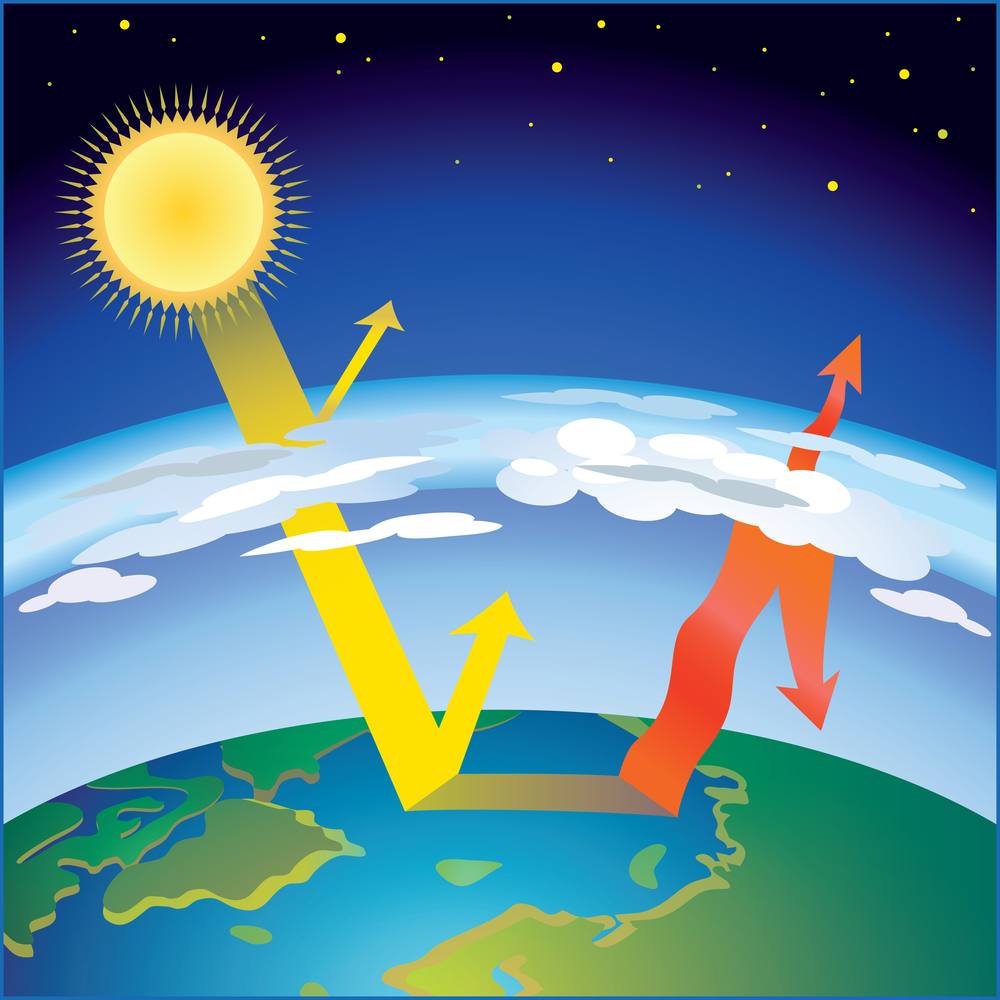
\includegraphics[width=7cm]{Figuras/estufa.jpg}
    \label{figura:estufa.jpeg}
    \end{figure}
    
\textit{Pera, pelo o que eu vi na televisão, o efeito estufa é prejudicial porque contribui para o aquecimento global, afinal ele é bom ou ruim?} \par
O que é ruim é o quanto nós humanos poluímos a atmosfera com gás carbônico. E é a presença desse gás na atmosfera que contribui para que as ondas solares fiquem presas aqui no planeta. Quanto mais jogamos ele no ar, menos as ondas são refletidas de volta para o espaço, e assim elas ficam aqui dentro nos esquentando.

\section{Aplicações no cotidiano}

\subsection{Óculos de visão noturna}
\paragraph{}
Alguns óculos de visão noturna permitem que a gente enxergue no escuro captando a radiação infravermelha do ambiente e gerando um termograma, que nada mais é do que uma imagem colorida que mostra onde está mais quente e onde está mais frio. Assim somos capazes de enxergar objetos e outras pessoas mesmo na escuridão.

\subsection{Câmeras térmicas}
\paragraph{}
Usando da mesma tecnologia que os óculos de visão noturna mencionados acima, essas câmeras convertem frequências que estão no espectro infravermelho para o espectro visível, assim conseguimos visualizar os objetos por meio do calor que eles emitem. Essas câmeras são úteis para encontrar pessoas ou animais em meio a vegetação, destroços ou esconderijos, além de poder encontrar falhas em equipamentos dependendo de onde estiver mais quente ou mais frio do que o normal.

\subsection{Controles remotos}
\paragraph{}
Quando você aperta um botão do seu controle remoto para mudar o canal da sua televisão, ele se comunica com a TV utilizando dos raios infravermelhos, se você apontar a câmera do seu celular para a lampadazinha na ponta do seu controle e apertar algum botão, você conseguirá enxergar os raios sendo emitidos. A seguir iremos explicar como que essa comunicação funciona.

\section{Controle infravermelho}
\label{ref:controle}
\paragraph{}
Agora vamos começar a falar sobre como podemos controlar o \textit{Sparki} utilizando o controle remoto, que vem junto com o kit. Ele funciona emitindo luz infravermelha a partir de sua lâmpada, luz essa que deve ser captada pelo sensor de infravermelho presente no \textit{Sparki}.

    \begin{figure}[h]
    \caption{Sensor de infravermelho}
     
    \centering 
    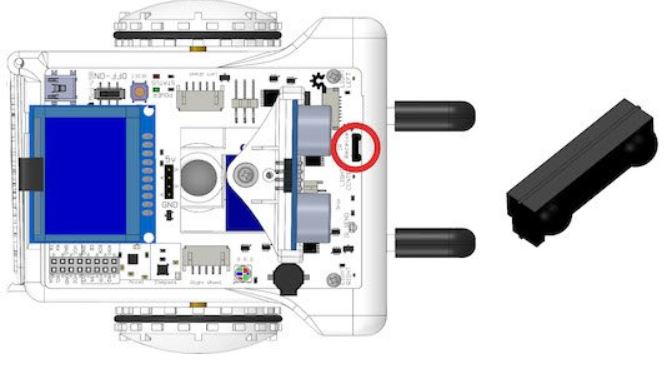
\includegraphics[width=7cm]{Figuras/sensor.JPG}
    \label{figura:sensor.jpeg}
    \end{figure}

\paragraph{}
Cada botão do controle remoto possui um padrão a ele relacionado, esse padrão representa quantas vezes a lâmpada do controle deve piscar e por quanto tempo, o sensor recebe esse padrão e o \textit{Sparki} é responsável por traduzir esse padrão para o botão correspondente. Para ficar mais fácil de entender é só lembrarmos do código Morse, onde cada letra e número é associado a um conjunto de pontos e traços. O que o controle remoto faz é parecido com a tradução de uma palavra em português  para código Morse, e depois o nosso robô deve saber ler essa palavra em código Morse e traduzir de volta para o português.

    \begin{center}
    \textcolor{mydarkblue}{\textbf{Atençao!}}
    \\ Os sinais infravermelhos não estão em código Morse, mencionamos ele apenas como forma de facilitar a compreensão. No geral, controles remotos têm padrões diferentes um do outro.
    \end{center}

\paragraph{}
Para facilitar a nossa vida, os criadores do \textit{Sparki} atribuíram a cada botão um número inteiro, como pode ser observado na Figura 8.4.

    \begin{figure}[h]
    \caption{Mapeamentos do controle}
     
    \centering 
    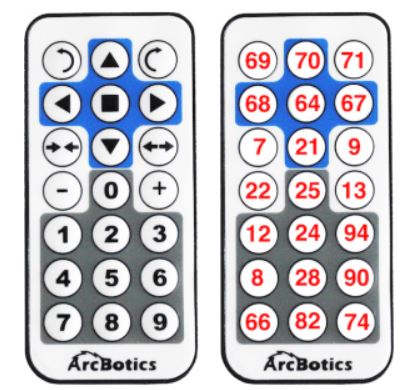
\includegraphics[width=5cm]{Figuras/controle.JPG}
    \label{figura:controle.jpeg}
    \end{figure}
    
\paragraph{}
Assim, quando utilizamos a função \lstinline[columns=fixed]{sparki.readIR()}, ela retorna o número inteiro associado ao botão que foi apertado. Para obtermos algum comando do controle devemos ter como base o seguinte código:

    \begin{lstlisting}[language=C]
#include <Sparki.h>;

int botao;

void setup()
{
}

void loop()
{
    botao = sparki.readIR();
}
\end{lstlisting}
    
Esta função salva na nossa variável inteira o número correspondente ao último botão que foi apertado antes dela ser chamada, caso não tenhamos apertado nenhum botão, ela irá salvar o valor \"-1".

\paragraph{}
Graças ao capítulo de \textit{if e else}, podemos escrever um algoritmo que executa uma atividade diferente para cada botão que for apertado, podemos controlar a movimentação do nosso robô da seguinte forma, por exemplo:

    \begin{lstlisting}[language=C]
#include <Sparki.h>;

int botao;

void setup()
{
}

void loop()
{
    botao = sparki.readIR();
    if(botao == 70)
    {
        sparki.moveStop();
        sparki.moveForward();
    }
    else if(botao == 67)
    {
        sparki.moveStop();
        sparki.moveRight();
    }
    else if(botao == 68)
    {
        sparki.moveStop();
        sparki.moveLeft();
    }
    else if(botao == 21)
    {
        sparki.moveStop();
        sparki.moveBackward();
    }
    else if(botao == 64)
    {
        sparki.moveStop();
    }
    delay(1000);
}
\end{lstlisting}

\section{Vetor de sensores infravermelhos}

\paragraph{}
Talvez você nunca tenha reparado, mas embaixo do \textit{Sparki} possui cinco retângulos pretos perto da garra, três no meio e um em cada canto. Esses retângulos são nada mais nada menos do que os sensores infravermelhos responsáveis por medir a \textbf{reflectância} da luz do chão abaixo dele (a reflectância de um corpo é a quantidade de luz que ele reflete).

\begin{comment}
Criar um card ilustrando o conceito de reflectância 
\end{comment}

    \begin{figure}[h]
    \caption{Os cinco sensores de reflectância infravermelha}
     
    \centering 
    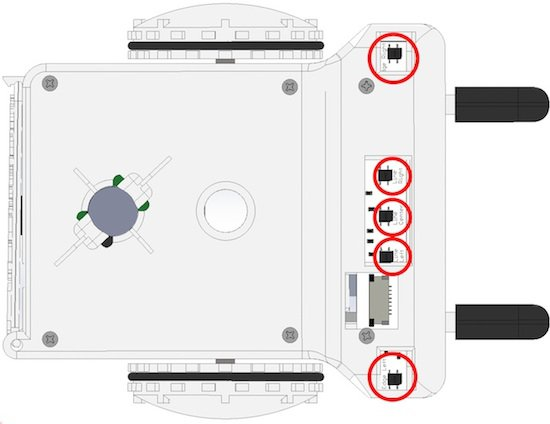
\includegraphics[width=8cm]{Figuras/vetor.jpg}
    \label{figura:vetor.jpeg}
    \end{figure}

\paragraph{}
Você já deve ter ouvido falar que a cor preta é a ausência de todas as cores, enquanto o branco é quando todas elas estão presentes, isso porque uma superfície preta absorve todas as frequências do espectro visível, enquanto o branco reflete todas de volta. Já uma superfície amarela, por exemplo, absorve todas as frequências menos a do amarelo, por isso vemos ela da cor amarela, porque foi a única frequência refletida para os nossos olhos. Como você já deve ter percebido, quando medimos a reflectância de uma superfície branca, certamente o valor será bem maior do que a de uma superfície preta.
\\~\\
\textit{Esses sensores então são utilizados para conseguirmos identificar quais são as cores que estão embaixo do Sparki?} \par
Essa é uma questão interessante! É sim possível diferenciar algumas cores pela sua reflectância. Mas até mesmo cores bem diferentes podem representar valores iguais ou muito semelhantes, e os sensores não são tão precisos e adequados para essa situação, certamente haverão muitos enganos. A verdadeira utilização deles é conseguir diferenciar superfícies mais escuras das mais claras, e isso é de extrema importância quando queremos fazer um exercício muito importante, um robô segue linhas, que normalmente anda por cima das linhas pretas num fundo branco.

\paragraph{}
É necessário certo cuidado ao utilizar esses sensores, porque uma mesma superfície pode retornar valores diferentes de reflectância, não podemos garantir que esteja tudo pintado no exato mesmo tom ou que haja a mesma incidência de luz em todo lugar, por isso quando mexemos com valores de reflectância devemos adotar \textbf{limiares}. Limiares são intervalos de valores que, embora diferentes um do outro, consideramos como sendo a mesma coisa, daremos como exemplo a separação das fases da vida, temos a fase infantil, adulta e terceira idade por exemplo, e dependendo da sua idade você irá se encaixar em uma dessas três fases.
\\~\\
\begin{tabular}{|c|c|c|c|c|c|}
    \cline{1-6}
     Limiares & 0 a 1 ano & 1 a 12 anos & 12 a 18 anos & 18 a 60 anos & 60 anos em diante \\
     \hline
     Classificação & Bebê & Criança & Adolescente & Adulto & Idoso \\
     \hline
\end{tabular}

\paragraph{}
A quantidade de limiares que vamos utilizar depende do problema do qual estamos tratando, na situação acima talvez fosse conveniente utilizar apenas 5 limiares, mas pode ser que em outra situação você teria que passar a incluir classificações como pré-adolescente ou ancião. Depois de determinados quais serão nossos limiares, podemos começar a coletar dados e então separá-los e classificá-los. Por exemplo, você tem 16 anos? Então você é um adolescente. Você tem 20 anos? Então você é um adulto. Você tem 14 anos, 7 meses, 2 semanas, 5 dias, 14 horas e meia de vida? Então você é considerado como sendo um adolescente também.

\paragraph{}
A importância do exemplo acima é fazer você entender que mais de um valor pode significar a mesma coisa, porque ao utilizar os sensores infravermelhos, você irá receber muitos valores de reflectância diferentes um do outro, e mesmo assim todos eles querem dizer que o chão é preto ou não, ou quem sabe só um pouco claro.

\subsection{Função}
\paragraph{}
Enfim, já está na hora de ensinarmos como você recebe esses valores de reflectância não é mesmo? Para cada um dos 5 sensores, existe uma função diferente que o ativa, ela nos retorna então um número \textbf{inteiro}, o qual devemos salvar numa variável inteira. As funções que ativam os sensores são: \lstinline[columns=fixed]{sparki.lineLeft()},\lstinline[columns=fixed]{sparki.lineRight()}, \lstinline[columns=fixed]{sparki.lineCenter()}, \lstinline[columns=fixed]{sparki.edgeLeft()} e \lstinline[columns=fixed]{sparki.edgeRight()}.

    \begin{center}
    \textcolor{mydarkblue}{\textbf{Para não esquecer!}}
    \\``Left'' traduzido para o português significa ``Esquerda'', ``Right'' significa ``Direita'' e ``Edge'' significa ``Borda ou Beira''.
    \end{center}
    
\paragraph{}
Caso estejamos interessados em saber se o \textit{Sparki} está pisando em cima de uma linha ou não, podemos escrever o seguinte código (vamos considerar que uma reflectância abaixo de 300 significa que a cor é preta e que acima disso a cor é branca).

    \begin{lstlisting}[language=C]
#include <Sparki.h>;

int limiar = 300, esquerda, centro, direita;

void setup()
{
sparki.clearLCD();
sparki.updateLCD();
}

void loop()
{
    esquerda = sparki.lineLeft();
    centro   = sparki.lineCenter();
    direita  = sparki.lineRight();
    delay(500);
if(esquerda < limiar || centro < limiar || direita < limiar)
{
    sparki.clearLCD();
    sparki.print("O Sparki está em cima de uma linha");
    sparki.updateLCD();
} else
{
    sparki.clearLCD();
    sparki.print("O Sparki NÃO está em cima de uma linha");
    sparki.updateLCD();
}
delay(500);
}
\end{lstlisting}

Nesse caso, se qualquer um dos 3 sensores do meio identificar a cor preta, estamos assumindo que o \textit{Sparki} está passando em cima de uma linha.
\\~\\
\textit{Calma lá! Mas afinal, por que esses sensores se chamam sensores infravermelhos? O que eles tem a ver com a luz infravermelha?} \par
Opa, desculpa! A razão do nome é porque junto com esses sensores, de baixo do \textit{Sparki}, nós temos LEDs (diodos emissores de luz) que emitem raios infravermelhos que serão refletidos pelo chão, e são esses raios que os sensores irão utilizar para medir a reflectância do chão.

\section{Exercícios}

    \question{Queremos que o \textit{Sparki} ande, pegue algum objeto com a sua garra e depois largue-o em algum outro lugar, escreva um algoritmo que permita que a gente, utilizando apenas o controle remoto, consiga fazer essa tarefa (se quiser você pode começar usando o código presente na seção \ref{ref:controle}). Suponha que a garra esteja inicialmente aberta.}

    \begin{center}
        \line(1,0){450}
        \vspace{0.2cm}   
        \line(1,0){450}
        \vspace{0.2cm}   
        \line(1,0){450}
        \vspace{0.2cm}   
        \line(1,0){450}
        \vspace{0.2cm}   
        \line(1,0){450}
        \vspace{0.4cm} 
    \end{center}

    \question{Escreva um código que faça com que o \textit{Sparki} faça contas de adição e de subtração com os números de 0 a 3 e que mostre o resultado da conta na tela LCD. Os números e a operação devem ser escolhidos apertando os botões do controle remoto.}
    
    \begin{center}
        \line(1,0){450}
        \vspace{0.2cm}   
        \line(1,0){450}
        \vspace{0.2cm}   
        \line(1,0){450}
        \vspace{0.2cm}   
        \line(1,0){450}
        \vspace{0.2cm}   
        \line(1,0){450}
        \vspace{0.4cm} 
    \end{center}

    \question{Escreva um código onde o \textit{Sparki} anda 5 centímetros em linha reta enquanto vai medindo a reflectância da superfície abaixo dele a cada centímetro e então calcula a reflectância média da superfície utilizando média aritmética.}
    
    \begin{center}
        \line(1,0){450}
        \vspace{0.2cm}   
        \line(1,0){450}
        \vspace{0.2cm}   
        \line(1,0){450}
        \vspace{0.2cm}   
        \line(1,0){450}
        \vspace{0.2cm}   
        \line(1,0){450}
        \vspace{0.4cm} 
    \end{center}

    \question{Utilizando dos sensores de reflectância infravermelha das bordas e o do centro, faça um programa onde o \textit{Sparki} ande em linha reta em cima de uma mesa e então PARE quando ele identificar que vai cair da mesa. Suponha que a mesa inteira seja da mesma cor e que quando a reflectância for menos do que 200, então passamos dos limites da mesa.}

    \begin{center}
        \line(1,0){450}
        \vspace{0.2cm}   
        \line(1,0){450}
        \vspace{0.2cm}   
        \line(1,0){450}
        \vspace{0.2cm}   
        \line(1,0){450}
        \vspace{0.2cm}   
        \line(1,0){450}
        \vspace{0.4cm} 
    \end{center}

    \challenge{\large{Desafio: escreva um programa onde o \textit{Sparki} seja capaz de andar por cima da faixa preta do percurso representado abaixo, fazendo com que ele fique andando em círculos (ele deve começar do traço no canto esquerdo inferior).}}

    \begin{figure}[h]
     
    \centering 
        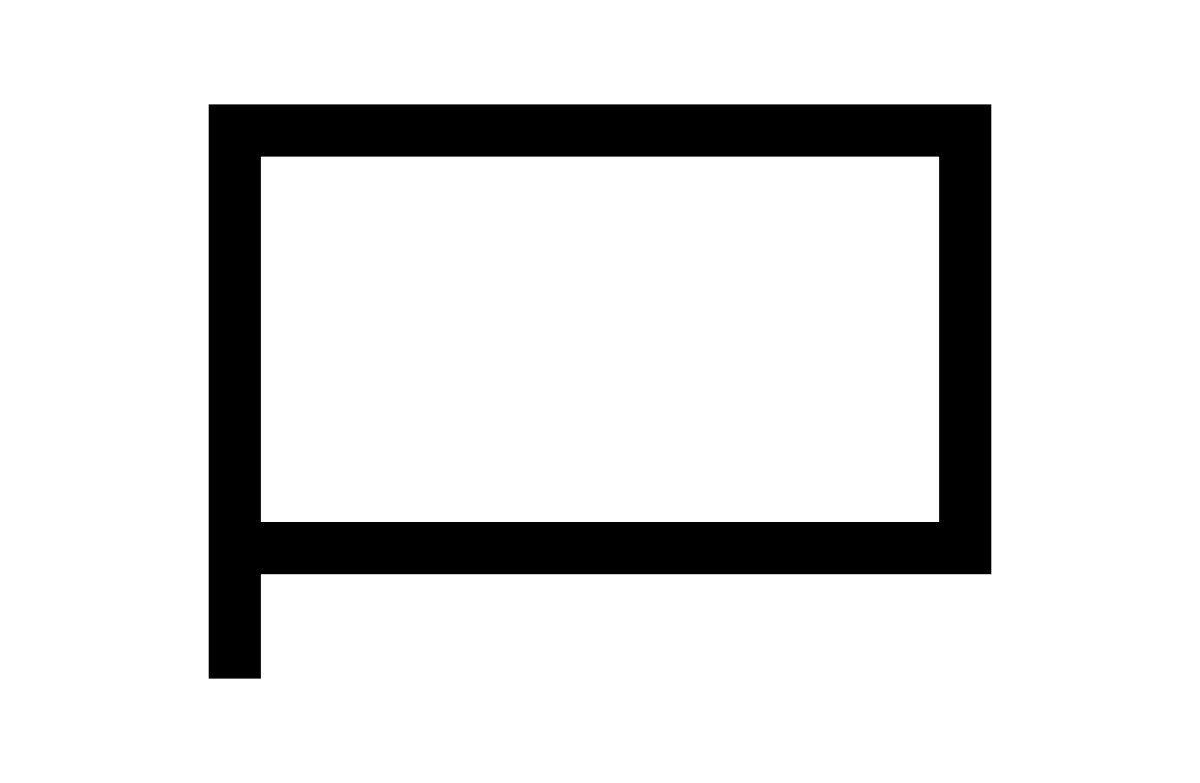
\includegraphics[width=5cm]{Figuras/trajeto.png}
        \label{figura:trajeto.jpeg}
    \end{figure}
    
    \begin{center}
        \line(1,0){450}
        \vspace{0.2cm}   
        \line(1,0){450}
        \vspace{0.2cm}   
        \line(1,0){450}
        \vspace{0.2cm}   
        \line(1,0){450}
        \vspace{0.2cm}   
        \line(1,0){450}
        \vspace{0.4cm} 
    \end{center}
\addcontentsline{toc}{chapter}{Gabarito}
\chapter*{Gabarito}

\addcontentsline{toc}{section}{Capítulo 1 - Afinal, o que é um robô?}
\section*{Capítulo 1 - Afinal, o que é um robô?}

    \subsection*{1)}
    Perguntar ao professor.
        \begin{multicols}{3}
            \begin{figure}[H]
            \caption{Praticar esportes}
     
            \centering 
            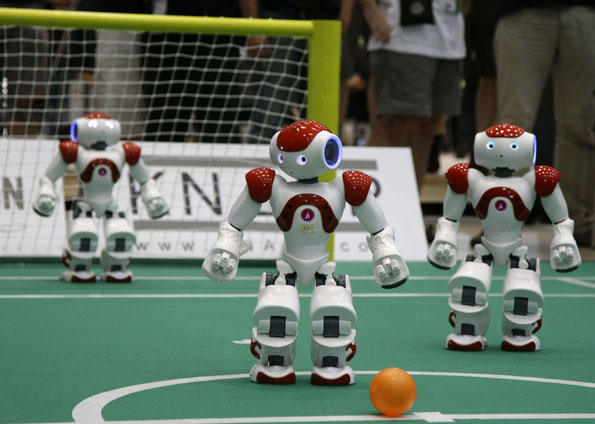
\includegraphics[width=5cm]{Figuras/NAO.jpg}
            \label{figura:NAO.jpeg}
            \end{figure}
        
            \begin{figure}[H]
            \caption{Robô que anda em terra e na água, pode ser utilizado para localizar coisas}
     
            \centering 
            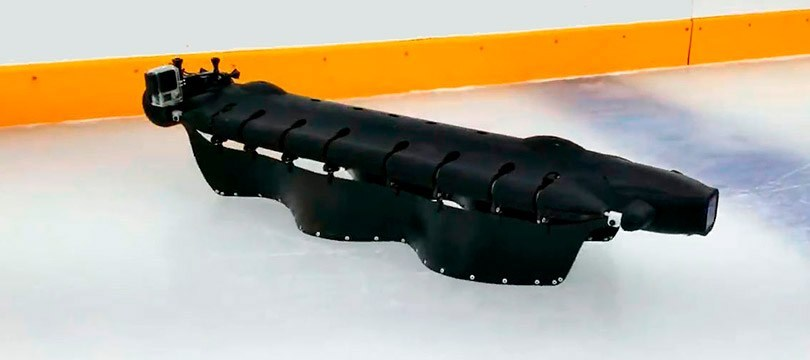
\includegraphics[width=5cm]{Figuras/anfibio.jpg}
            \label{figura:anfibio.jpeg}
            \end{figure}

            \begin{figure}[H]
            \caption{Sophie, estudos sobre inteligência artificial}
     
            \centering 
            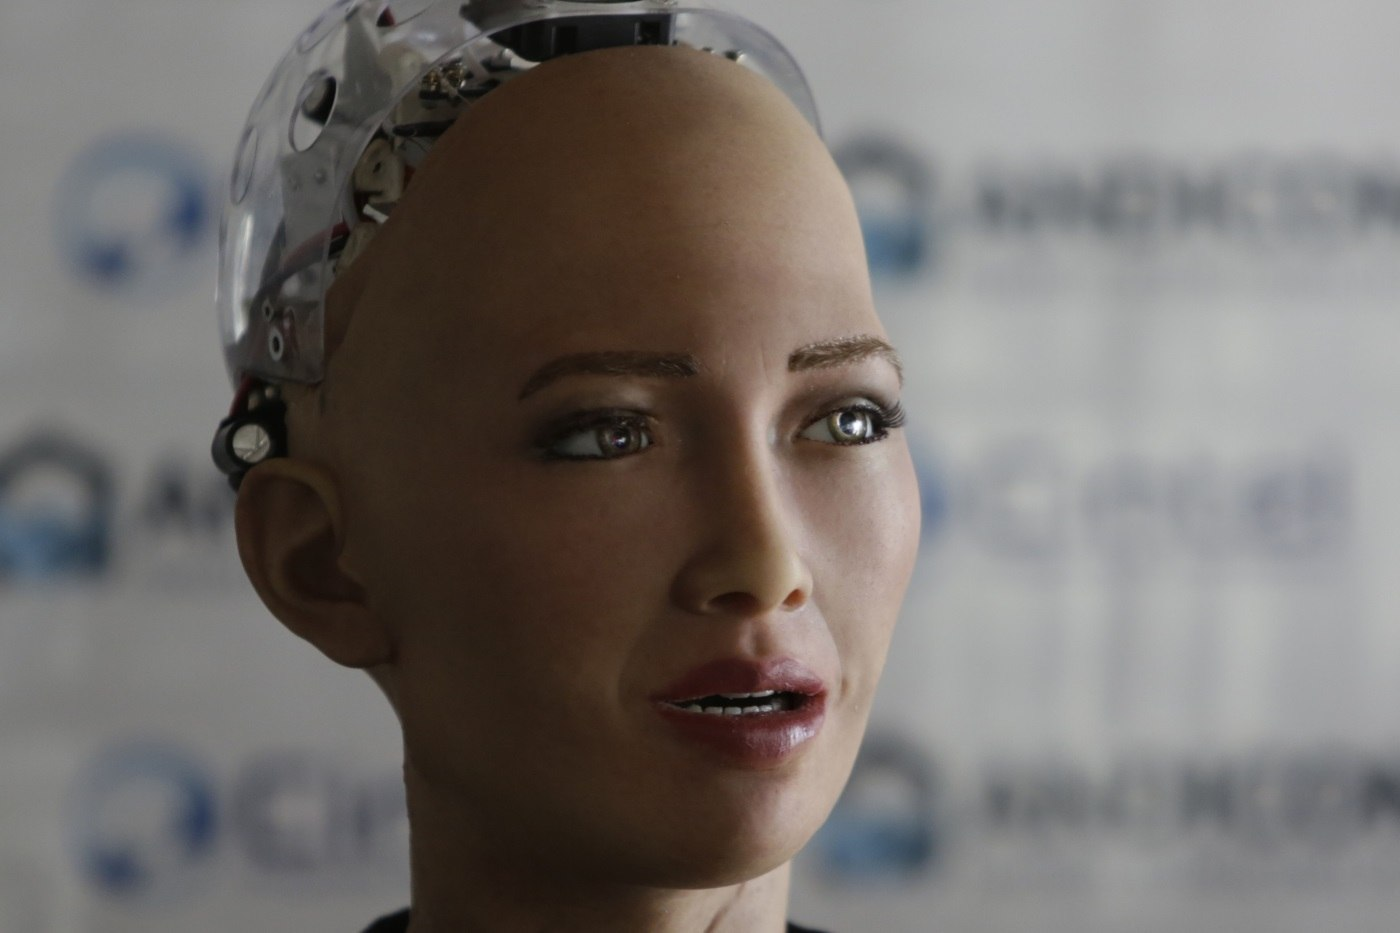
\includegraphics[width=6cm]{Figuras/sophie.jpeg}
            \label{figura:sophie.jpeg}
            \end{figure}
        \end{multicols}
        
     \subsection*{2)}
        Não, termômetros não são capazes de tomar decisões, de agir sobre o meio, ele é somente uma ferramenta para calcular e visualizar a temperatura ambiente.
        
    \subsection*{3)} Perguntar ao professor.
        
    \subsection*{4)}
        A geladeira sabe quando a porta está aberta e quando está fechada, e nisso decide se acende ou apaga a luz de dentro dela, porém isso não passa apenas de algum circuito lógico. Uma boneca que fala ou se mexe sozinha é bem "robótica" por dentro, mas é incapaz de perceber os seus arredores e realizar ações não repetitivas (tenha certeza que o fabricante disse que a boneca deveria se mexer, caso não venha explicitado, pode ser caso de assombração!).
        
    \subsection*{\textbf{Desafio}}
        Perguntar ao professor.
        

\addcontentsline{toc}{section}{Capítulo 2 - Algoritmos e fluxograma}        
\section*{Capítulo 2 - Algoritmos e fluxograma}

    \subsection*{1)} Perguntar ao professor.
    
    \subsection*{2)} Letra a.
    
    \subsection*{3)} Existem varias soluções corretas, aqui vai uma sugestão, busque sempre ser detalhista.
        \begin{figure}[H]
        \centering
        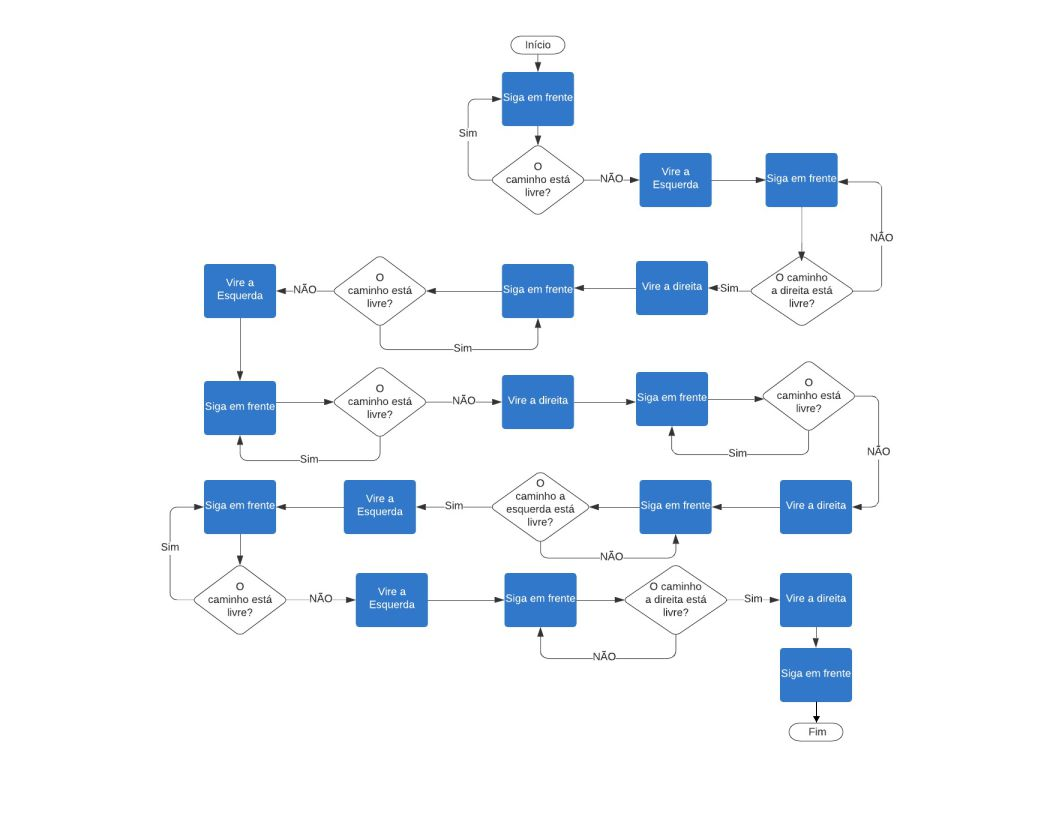
\includegraphics[width=18cm]{Figuras/sollab.jpg}
        \label{figura:solução.jpg}
        \end{figure}
    
\addcontentsline{toc}{section}{Capítulo 3 - Tela LCD}      
\section*{Capítulo 3 - Tela LCD}
    
    \subsection*{1)} Para descobrir o meio da tela, basta dividir as dimensões da tela LCD por dois, logo, o ponto central terá as seguintes coordenadas: \\ x = 128 / 2 = 64 \\ y = 64 / 2 = 32
    

    \lstinputlisting[language=C] {codigos_gabarito/capitulo_3/exercicio-3.1.c}
    
    \subsection*{2)} Letra d.
    
    \subsection*{3)} 
    
    %Ajustar o recuo da esquerda.
     a) 10 pixels.\\
    \indent b) 25 pixels.

    \subsection*{Desafio) Perguntar ao professor.}

\addcontentsline{toc}{section}{Capítulo 4 - Movimentação} 
\section*{Capítulo 4 - Movimentação}

    \subsection*{1)}
    Letra c.
    
    \subsection*{2) (Existe mais de uma solução para este exercício)}

 \lstinputlisting[language=C]{codigos_gabarito/capitulo_4/exercicio-2.c}

    \textsl{Como a distância a ser percorrida pelo robô é equivalente ao lado do quadrado, o valor dentro dos parênteses da função ``sparki.moveForward()'' é 5.}
    
    \subsection*{3) (Existe mais de uma solução para este exercício)} 
    
     \lstinputlisting[language=C]{codigos_gabarito/capitulo_4/exercicio-3.c}
    
    \subsection*{4)}
    Letra d.
    
    \subsection*{5)}
    
 \lstinputlisting[language=C]{codigos_gabarito/capitulo_4/exercicio-5.c}
 
    \subsection*{6)}
    \textsl{Este código abre totalmente as garras e depois as fecha durante 1 segundo. Poderia simular as garras pegando um objeto.}
    
    \subsection*{Desafio) Perguntar ao professor.}
    
\addcontentsline{toc}{section}{Capítulo 5 - Variáveis} 
\section*{Capítulo 5 - Variáveis}

    \subsection*{1)}
 \lstinputlisting[language=C]{codigos_gabarito/capitulo_5/exercicio-1.c}
 
    \subsection*{2)}
 \lstinputlisting[language=C]{codigos_gabarito/capitulo_5/exercicio-2.c}


 %   \subsection*{3)}
 %   \begin{lstlisting}[language=C]

%#include <Sparki.h>;

%int distancia;

%void setup()
%{
%}

%void loop()
%{
%    distancia = sparki.ping();
%    distancia -=10;
%    sparki.moveForward(distancia);
%}
%\end{lstlisting}

%   } não sei se isso deveria estar aq, mas caso fosse para estar então não apaguei
    
    \subsection*{Desafio) Perguntar ao professor.}

 \lstinputlisting[language=C]{codigos_gabarito/capitulo_5/desafio.c}

\addcontentsline{toc}{section}{Capítulo 6 - Ultrassom} 
\section*{Capítulo 6 - Ultrassom}

    \subsection*{1)}
    
        Conhecendo a velocidade do som, que é aproximadamente 340 m/s, nós sabemos quantos metros o som percorre em 1 segundo.
        Se conhecermos também quanto tempo levou para a onda ir e voltar, podemos fazer uma \textbf{regra de três} para descobrir quantos metros a onda andou.
        Ou seja, o som faz: 
        \par
        \textbf{340} metros => \textbf{1} segundo 
        \par
        \textbf{x} metros => \textbf{t} segundo(s) \par
        Sendo \textbf{x} a quantidade de metros que a onda andou e \textbf{t} quantos segundos foram necessários para a onda fazer esse trajeto.
        Então, podemos achar \textbf{x} multiplicando as diagonais da regra de 3 e igualando-as, assim: 
        \par
        \textbf{340} . \textbf{t} = \textbf{x} . \textbf{1} 
        \par
        Agora, isolamos o \textbf{x}:
        \par
        \textbf{x} = 340t
        \par
        Mas devemos levar em consideração que a onda vai até o objeto e volta até o sensor, por isso a distância do sensor até o objeto é metade do \textbf{x} encontrado:
        \par
        \textbf{x} = 340t/2 = 170t
        \par
        E esse é o nosso resultado!
    
    \subsection*{2)}
    
 \lstinputlisting[language=C]{codigos_gabarito/capitulo_6/exercicio-2.c}

    \subsection*{3)}
    
 \lstinputlisting[language=C]{codigos_gabarito/capitulo_6/exercicio-3.c}

    
    \subsection*{4)}
    
 \lstinputlisting[language=C]{codigos_gabarito/capitulo_6/exercicio-4.c}

    
    \subsection*{Desafio) Perguntar ao professor.}

\addcontentsline{toc}{section}{Capítulo 7 - If e Else}
\section*{Capítulo 7 - If e Else}

    \subsection*{1)} x = 2; y = 1; Falso.

    \subsection*{2)} Verdadeiro; Verdadeiro.

    \subsection*{3)} Verdadeiro.

    \subsection*{4)} Letra b.
    
    \subsection*{5) (Existe mais de uma solução para este exercício)}
    
 \lstinputlisting[language=C]{codigos_gabarito/capitulo_7/exercicio-5.c}
    
    \subsection*{6)}
    
 \lstinputlisting[language=C]{codigos_gabarito/capitulo_7/exercicio-6.c}


    \subsection*{Desafio) Em caso de dúvidas, perguntar ao professor.}

\addcontentsline{toc}{section}{Capítulo 8 - Infravermelho}
\section*{Capítulo 8 - Infravermelho}

    \subsection*{1)}
    A resposta a seguir é apenas um exemplo, pode-se utilizar de quaisquer botões disponíveis para controlar o robô.
    
 \lstinputlisting[language=C]{codigos_gabarito/capitulo_8/exercicio-1.c}

    
    \subsection*{2)}
    
 \lstinputlisting[language=C]{codigos_gabarito/capitulo_8/exercicio-2.c}
 
    O passo 1 do programa é quando recebemos o primeiro número da conta, no segundo passo devemos definir se a operação é de adição ou de subtração, no terceiro passo escolhemos o segundo número e por último fazemos os cálculos e mostramos o resultado na tela LCD. Caso o usuário não aperte os botões corretos, o programa detecta a falha e repete o último passo.
    
    \subsection*{3)}
 
 \lstinputlisting[language=C]{codigos_gabarito/capitulo_8/exercicio-3.c}

    
    \subsection*{4)}
    
 \lstinputlisting[language=C]{codigos_gabarito/capitulo_8/exercicio-4.c}

    
    \subsection*{Desafio) Perguntar ao professor.}
    
\addcontentsline{toc}{chapter}{Bibliografia}
\chapter*{Bibliografia}

\section*{O que é um robô?}

\noindent Figura \ref{figura:roomba.jpeg}: https://cdn.vox-cdn.com/thumbor/xpZtjkhdMzkTSOPW9GPcKSev-tE=/0x0:2040x1360/\\1200x800/filters:focal(826x814:1152x1140)/cdn.vox-cdn.com/uploads/chorus\_image/image/62367388/\\dseifert\_180924\_2969\_0039.0.jpg

\section*{Algoritmos e Fluxogramas}

\noindent Figura \ref{figura:Pipoca.jpeg}: https://www.lucidchart.com/
\\~\\
Figura \ref{figura:formas.jpeg}: https://certificacaoiso.com.br/wp-content/uploads/2017/07/s%C3%ADmbolos_fluxograma.jpg
\\~\\
Figura \ref{figura:torre.jpeg}: https://images-na.ssl-images-amazon.com/images/I/51gEuCb-MjL.\_AC\_SX425\_.jpg
\\~\\
Figura \ref{figura:Labirinto.jpeg}: https://www.vecteezy.com/free-vector/labirinto

\section*{Tela LCD}

\noindent Figura \ref{figura:LCD_Diagram1.jpg}: http://arcbotics.com/wp-content/uploads//2014/01/LCD-Diagram.jpg
\\~\\
Figura \ref{figura:Top_LCD1.jpeg}: http://arcbotics.com/wp-content/uploads//2015/12/Top-LCD.jpeg

\section*{Movimentação}

\noindent Figura \ref{figura:movimentation_for_back.png}: http://arcbotics.com/wp-content/uploads/2015/12/SparkiMovementB31.png
\\~\\
Figura \ref{figura:rotation.png}: http://arcbotics.com/wp-content/uploads/2015/12/movingTheRobotRightCenter.png
\\~\\
Figura \ref{figura:movingTheRobotmoveLeft.png}: http://arcbotics.com/wp-content/uploads/2015/12/movingTheRobot.moveLeft.png

\section*{Ultrassom}

\noindent Figura \ref{figura:ultrassom.jpeg}: https://uploads.filipeflop.com/2017/07/9SS01-3.jpg
\\~\\
Figura \ref{figura:onda.jpeg}: https://uploads.filipeflop.com/2011/07/HC\_SR04\_Trigger\_Echo.jpg
\\~\\
Figura \ref{figura:servo.jpeg}: https://www.vidadesilicio.com.br/media/catalog/product/cache/2/thumbnail/450x450/\\9df78eab33525d08d6e5fb8d27136e95/8/5/850xn\_3\_\_1.jpg

\section*{Infravermelho}

\noindent Figura \ref{figura:espectro.jpeg}: https://s3.static.brasilescola.uol.com.br/img/2019/05/espectro-visivel.jpg
\\~\\
Figura \ref{figura:estufa.jpeg}: https://static.significados.com.br/foto/efeito-estufa-e-aquecimento-global-significados.jpg
\\~\\
Figura \ref{figura:sensor.jpeg}: http://arcbotics.com/wp-content/uploads/2015/12/Remote\_Top.jpg
\\~\\
Figura \ref{figura:controle.jpeg}: http://arcbotics.com/wp-content/uploads/2015/12/Remote-Cleared-297x3001.png
\\~\\
Figura \ref{figura:vetor.jpeg}: http://arcbotics.com/wp-content/uploads/2015/12/Sparki\_Underside2.jpg
\\~\\

\section*{Gabarito}

\noindent Figura \ref{figura:NAO.jpeg}:https://g1.globo.com/Noticias/Tecnologia/foto/0,,21262370-FMM,00.jpg 
\\~\\
Figura \ref{figura:anfibio.jpeg}: https://i1.wp.com/geekness.com.br/wp-content/uploads/2018/12/Robo-Anfibio-Velox-GEEKNESS-1.jpg?fit=810\%2C360\&ssl=1
\\~\\
Figura \ref{figura:sophie.jpeg}: https://img.r7.com/images/robo-sophia-1400-31082018123425994?\\dimensions=600x315\&crop\_position=c


% Referências
%\bibliographystyle{abbrv} 
%\bibliography{references} % nome do arquivo
\end{document}